\documentclass[11pt,a4paper]{article}

\usepackage[margin=1in]{geometry}
\usepackage[T1]{fontenc}
\usepackage{lmodern}
\usepackage{amsmath,amssymb,amsthm}
\usepackage{mathtools}
\usepackage[protrusion=true,expansion=false]{microtype}
\usepackage{hyperref}
\usepackage{booktabs}
\usepackage{tabularx}
\usepackage{graphicx}
\usepackage{xcolor}
\usepackage{enumitem}
\usepackage{caption}
\usepackage{tikz}
\usepackage{pgfplots}
\pgfplotsset{compat=1.18}
\usepackage[numbers,sort&compress]{natbib}
\usepackage{url}

\hypersetup{
  pdftitle={ECC2K-130 on Commodity Hardware: A Measured Frobenius-Class Pollard Rho Campaign},
  pdfauthor={Anonymous},
  colorlinks=true,
  linkcolor=blue!50!black,
  citecolor=blue!50!black,
  urlcolor=blue!50!black,
}

\newtheorem{theorem}{Theorem}[section]
\newtheorem{lemma}[theorem]{Lemma}
\newtheorem{proposition}[theorem]{Proposition}
\theoremstyle{definition}
\newtheorem{definition}[theorem]{Definition}
\newtheorem{remark}[theorem]{Remark}

\newcommand{\FF}{\mathbb{F}}
\newcommand{\ZZ}{\mathbb{Z}}
\newcommand{\QQ}{\mathbb{Q}}
\newcommand{\HW}{\operatorname{HW}}
\renewcommand{\gcd}{\operatorname{gcd}}
\newcommand{\Bs}{\,\mathrm{B/s}}
\newcommand{\thisrepo}{\texttt{crypto}}
\newcommand{\sibling}{\texttt{cryptanalysis}}
% Footnote a number to a repository artefact. Paths without a repo prefix
% are in this repository; paths prefixed cryptanalysis: are in the sibling
% library and paths prefixed autoresearcher: in the research-ledger repository.
\newcommand{\art}[1]{\footnote{\texttt{\detokenize{#1}}.}}

\title{ECC2K-130 on Commodity Hardware:\\
       A Measured Frobenius-Class Pollard Rho Campaign}
% Anonymized for double-blind submission.  Author block restored
% for camera-ready / preprint release; see README.md.
\author{Anonymous}
\date{}

\begin{document}
\maketitle
\emergencystretch=2em

\begin{abstract}
\input{abstract.txt}
\end{abstract}

\tableofcontents
\clearpage

\section{Introduction}
\label{sec:intro}

In 1997 Certicom published a list of elliptic-curve discrete
logarithm challenges~\cite{certicom1997}. The Koblitz challenges
ECC2K-95, ECC2K-108 and ECC2K-130 ask for $k$ with $Q=[k]P$ on
$y^2+xy=x^3+1$ over $\FF_{2^{97}}$, $\FF_{2^{109}}$ and $\FF_{2^{131}}$.
Harley's group solved ECC2K-95 in 1998~\cite{harley1998} and ECC2K-108
in 2000; ECC2K-130 is open. In 2009 a consortium of twenty authors
published the arithmetic, the iteration function and the per-platform
throughput of a planned attack~\cite{bailey2009,bailey2009sharcs,bos2010cell,fan2010fpga}
and estimated the work at $2^{60.9}$ iterations. The attack did not
complete.

This paper is a measured account of a second attempt, built from
scratch on hardware that did not exist in 2009 and documented to a
standard the first attempt's reports set: every rate paired against
an adjacent control on the same allocation, every boundary written
down before the kernel was tuned toward it, every claim footnoted to a
file in the repository that holds it. The work is not an advance on
the generic-group floor and the paper does not say it is. What it
reports is the cost of one step, measured on GPUs, CPUs and an FPGA,
the number of steps, measured on toy curves of the same family and
extrapolated, and a campaign that walked $2^{56.4}$ of the $2^{60.9}$
before its fleet was taken away.

\paragraph{Contributions.}
\begin{itemize}[leftmargin=1.2em,itemsep=0.3em]
\item A code generator that builds every field routine from one
  symmetric-vector model of $\FF_{2^{131}}$ and checks it before
  emitting it; a bitsliced backend at every word width from 64 to 512
  lanes and a packed CUDA backend with native carry-less products;
  bit-for-bit compatible records across all of them and a VHDL engine
  (Sections~\ref{sec:curve}, \ref{sec:arith}).
\item Three iteration functions on the $\langle\sigma,-1\rangle$
  classes, with the walk constant measured on toy Koblitz curves and
  extrapolated: $2^{60.91}$--$2^{60.92}$ iterations for the campaign's
  walk, with the table walk's fruitless cycles measured, priced and
  repaired (Section~\ref{sec:walk}).
\item A GPU ledger of sixteen paired rungs from $0.85$ to
  $14.64$~B/s on one RTX~PRO~6000, a table walk at $20.08$~B/s, a
  twelve-SKU survey, a roofline, and a floor derived from the
  carry-less unit before tuning that rules out $28$~B/s on one card;
  with every declined candidate and its ratio (Section~\ref{sec:gpu}).
\item A pipelined-Karatsuba FPGA engine measured at $8.25$~G steps/s
  on one AWS F2, within a pre-board estimate of $5$--$12$
  (Section~\ref{sec:fpga}).
\item A live campaign: configuration, the calibration of the
  distinguished-point interval (and the retraction of a wrong one),
  the storage and replay protocol, fleet economics, and the state at
  $367$~M points (Section~\ref{sec:campaign}).
\item The structural alternatives priced in the same unit and found
  wanting: index calculus on the Koblitz curve at $10^7\times$ rho, and
  point decomposition $35$--$51$ bits short of its budget
  (Section~\ref{sec:alternatives}).
\end{itemize}

\paragraph{Method.} The reporting rule of the repository, stated
here once, governs every section~\cite{ecdlppaper}. A change is
measured as a ratio to a boundary that was written down first: a
floor from a counting or pipe argument that the method cannot cross,
or a reference, the best existing method on the same instance in the
same unit. Every change is classified by what moved: an
\emph{advance} lowers the ratio to the floor; \emph{engineering}
lowers the cost with the ratio to the floor flat; \emph{relabelling}
lowers a headline while the total rises; \emph{accounting} changes a
number without changing the algorithm. All four are committed, and
every row in this paper is one of the last three. A rate quoted
without its paired control, its hardware and its geometry is the
unit mistake this paper tries hardest not to make, and
Sections~\ref{sec:ledger} and \ref{sec:campaign-interval} each record
one instance where an earlier draft of the repository made it.

\paragraph{Two repositories.} The campaign lives in a study
repository, \thisrepo, whose notes this paper cites by path. A
sibling library, \sibling, holds an independent C golden model of the
same field, a digit-serial FPGA core with no vendor timing, an import
of the $20$~B/s GPU client with its own host re-walk, and the
boundary ledger for index calculus; its companion
paper~\cite{ecdlppaper} places ECC2K-130 among other discrete-logarithm
measurements in the unit $S=\text{ops}/\sqrt n$. Paths prefixed
\texttt{cryptanalysis:} are in that library; two evidence records cited
in Section~\ref{sec:alternatives} live in a third repository, the
research ledger, and are prefixed \texttt{autoresearcher:}.

\paragraph{What is not claimed.} No logarithm has been recovered on
the challenge curve and none is expected from the corpus so far. No
rate in this paper is quoted for hardware that was not measured; the
L40S collection rate, the RTX~PRO~4500 collection rate under the
bridge map and the G7e instance family are unmeasured and are said to
be. Projections (the $7.2$--$7.4$~B/s fused build on the 4500, the
table walk's $0.81$--$0.86$ cost per solve, the 136- and 144-engine F2
images) are labelled as projections where they appear.

\section{The curve, the field and the golden model}
\label{sec:curve}

ECC2K-130 is the Certicom challenge~\cite{certicom1997}
\[
  E:\ y^2 + xy = x^3 + 1 \qquad\text{over }\FF_{2^{131}},
\]
a Koblitz curve~\cite{koblitz1992} defined over $\FF_2$, with group
order $4\cdot\ell$,
\[
  \ell = 680564733841876926932320129493409985129,
\]
a 129-bit prime.\art{ecc2k130/README.md, ``The problems''} The
challenge asks for $k$ with $Q=[k]P$ for published $P$ and $Q$ of
order $\ell$. It has been open since 1997; the 2009 consortium
estimate of the work is $2^{60.9}$ iterations of a
Frobenius-equivariant walk~\cite{bailey2009}, and
Section~\ref{sec:walk-constant} measures this paper's walk at
$2^{60.91}$--$2^{60.92}$ on completed trails.

The curve is identified rather than trusted. $E(\FF_2)$ has four
points, so the Frobenius trace is $t=-1$ and the Koblitz recursion
$s_m = t\,s_{m-1} - 2 s_{m-2}$ gives $\#E(\FF_{2^{131}}) = 2^{131}+1-s_{131}
= 4\ell$. The sibling library's test suite checks the two facts that
make this \emph{this} curve, on random points multiplied by the
cofactor: $\sigma^2+\sigma+2=0$, where $\sigma(x,y)=(x^2,y^2)$ is the
Frobenius, and $\ell\cdot
R=\mathcal{O}$.\art{cryptanalysis:fpga/README.md}\art{cryptanalysis:fpga/model/ecc2k130_test.c}
The published challenge point converts out of the normal basis back
to Certicom's polynomial-basis hex, \texttt{05 1C99BFA6 F18DE467
C80C23B9 8C7994AA}.\art{ecc2k130/README.md, ``Validation''}

\subsection{A type-II optimal normal basis}
\label{sec:onb}

$2\cdot131+1=263$ is prime and $2$ has order $131$ modulo $263$, so
$\FF_{2^{131}}$ has a type-II optimal normal basis. With $\zeta$ a
primitive $263$rd root of unity the basis is
$\gamma_i = \zeta^i + \zeta^{-i}$, $i=1,\ldots,131$, and an element is a
131-bit vector. Every design in this paper, on every platform, is
built on three consequences.\art{ecc2k130/README.md, ``Field representation''}

\begin{center}
\small
\begin{tabular}{@{}p{0.42\textwidth}p{0.48\textwidth}@{}}
\toprule
fact & consequence \\
\midrule
$\gamma_i\gamma_j = \gamma_{i+j} + \gamma_{i-j}$
  (indices folded by $\gamma_{263-k}=\gamma_k$, $\gamma_0=0$)
  & a product is a cyclic convolution of two symmetric 263-bit
    vectors, or, after a Bernstein--Lange change of basis, a
    polynomial product with no reduction step \\
$\gamma_i^2 = \gamma_{2i \bmod 263}$
  & squaring is the index permutation $i\mapsto\mathrm{fold}(2i)$:
    free when loops are unrolled, wiring on an FPGA, so every
    Frobenius power $\sigma^k$ costs nothing \\
the Hamming weight of the vector is invariant under $\sigma$ and under
  negation $-(x,y)=(x,x+y)$
  & the iteration's branch selector and the distinguished-point
    predicate are functions on $\langle\sigma,-1\rangle$-classes that
    read the vector the hardware already holds \\
\bottomrule
\end{tabular}
\end{center}

\subsection{The golden model}
\label{sec:golden}

None of this is taken on trust. The code generator models the field
as the symmetric vectors over $\ZZ/263\ZZ$ modulo the all-ones vector,
with multiplication as cyclic convolution: a complete and obviously
correct model of $\FF_{2^{131}}$, and the one every generated routine is checked against on 64 random
inputs before it is written out.\art{ecc2k130/codegen/field.py}\art{ecc2k130/codegen/gen.py} The bitsliced multiply, square,
inverse, $\sigma^7$ and Hamming weight are differentially tested
against a reference implementation that shares no code with them;
the iteration function is checked to commute with Frobenius and with
negation; the collision solver recovers a planted logarithm; the
distinguished-point comparison is checked exhaustively over all
weights and cutoffs. \texttt{make test} runs 52 such checks across
$\mathrm{GF}(2^{23})$, $\mathrm{GF}(2^{41})$, $\mathrm{GF}(2^{83})$ and
$\mathrm{GF}(2^{131})$.\art{ecc2k130/README.md, ``Validation''}

The same model is the oracle for every other platform. The VHDL
engine's reference script imports it directly and proves the
basis-change maps, the multiplier route, $\sigma^j$, the inversion
chain and a full step before emitting test vectors
(Section~\ref{sec:fpga}).\art{hdl/ecc2k130/ecc2k_ref.py} The sibling
library's independent C model of the same field and curve
(\texttt{cryptanalysis:fpga/model/ecc2k130.c}) was built separately
and re-walks every GPU report that library imports; agreement between
the two models on the same records is equality of 131-bit vectors in
the same permuted basis, not equivalence up to a basis
change~\cite{ecdlppaper}.

Longer runs check the reporting path rather than the algebra. On
$\mathrm{GF}(2^{83})$, $12.6$~M iterations produced 172 distinguished
points, within $30\%$ of the predicted rate, and 60 of them were
recomputed from their seeds by the reference with no mismatch,
including walks that had been restarted. On the challenge curve
itself, with the cutoff loosened from 34 to 50 so that points appear,
$3.1$~M iterations produced $12{,}368$ reports, 25 of which were
recomputed and matched exactly.\art{ecc2k130/README.md, ``Validation''}

\subsection{ECC2K-95 as the end-to-end control}
\label{sec:ecc2k95}

ECC2K-95 is the retired Certicom challenge on the same curve equation
over $\FF_{2^{97}} = \FF_2[t]/(t^{97}+t^6+1)$, group order $4\ell$ with
$\ell = 39614081257132074233778707191$ a 95-bit prime, solved by
Harley and collaborators in 1998~\cite{harley1998}. $2\cdot97+1=195$ is
composite, so there is no type-II optimal normal basis; the client
runs a polynomial-basis backend with the orbit-invariant weight taken
through one generated linear map into a normal basis, which is the
arrangement Harley's own client used.\art{ecc2k130/README.md, ``ECC2K-130 and ECC2K-95''}

The parameters were recovered from Harley's surviving client source
and the generator refuses to emit the curve unless both points lie on
it, both have order $\ell$, and the published answer
\[
  k = 37837308472231540269443981458
\]
satisfies $[k]P=Q$. Expected work is about $2^{44}$ iterations;
Harley's group measured $2.16\cdot10^{13}$ against the
$1.79\cdot10^{13}$ this walk predicts from
$\sqrt{\pi\ell/(4m)}$.\art{ecc2k130/README.md, ``The problems''} Per
iteration the polynomial-basis field is about $1.9\times$ cheaper
than $\mathrm{GF}(2^{131})$ in the normal basis (about $32{,}000$
against $60{,}000$ bitsliced instructions), so ECC2K-95 is a
few GPU-hours where ECC2K-130 is GPU-centuries: a real end-to-end
test of the whole pipeline at a scale that completes.
\art{ecc2k130/README.md, ``ECC2K-95''} The repository's separate
ECC2K-95 CUDA kernel has run only through CPU emulation, where it
recovers 21-bit and 40-bit toy logarithms at $0.94\times$ and
$1.32\times$ its own prediction, and is not a throughput
claim.\art{gpu/ecc2k/README.md}

\section{The walk}
\label{sec:walk}

Pollard's rho~\cite{pollard1978} in the parallel collision-search
form of van Oorschot and Wiener~\cite{vanoorschot1999} walks many
pseudo-random trails through the group, reports the distinguished
points it passes, and solves the logarithm when two trails meet. On a
Koblitz curve the Frobenius $\sigma$ and negation generate a group of
automorphisms of order $2m=262$ that act on $\langle P\rangle$, and a
walk defined on the orbits of that group needs $\sqrt{262}\approx16.2$
times fewer steps~\cite{wienerzuccherato1998,glv2000,duursma1999}.
The expected number of classes visited before a collision on
$N=(\ell-1)/262$ classes is $\sqrt{\pi N/2}$, which is $2^{60.809}$
here.\art{ecc2k130/WALK-CONSTANT.md, §1} Every walk in this paper is
a map on those classes; what differs between them is how the class
action is respected and how much each step costs.

\subsection{The $\sigma$-walk}
\label{sec:walk-sigma}

The campaign walks the map of Bailey et al.~\cite{bailey2009}:
\begin{align*}
  j &= 3 + \bigl((\HW(x_R) \gg 1) \bmod 8\bigr) \in [3,10],\\
  R' &= \sigma^j(R) + R,\\
  \text{distinguished} &\iff \HW(x_R)\le w,
\end{align*}
with $w=34$ in the client's default and $w=32$ in the live campaign.
Because the weight is a class invariant, $f(\sigma R)=\sigma f(R)$ and
$f(-R)=-f(R)$, so the map descends to classes without any canonical
representative being computed inside the loop. The division by two
in the selector is load-bearing: $x$-coordinates of subgroup points
have even weight, and a selector on the raw weight would use only
four of the eight branches.\art{gpu/ecc2k/README.md}

One step is one affine addition: one inversion, two multiplications
and a free Frobenius, since $\sigma^j$ is wiring. As a scalar the step
is $R\mapsto[1+s^j]R$ where $s$ is the root of $s^2+s+2=0$ that
$\sigma$ realises on $\langle P\rangle$. The $\sigma^j$ selection is
branch-free: three conditional squarings, each one \texttt{LOP3} per
word, and $j$ is never materialised.\art{ecc2k130/README.md, ``Iteration function''}

No coefficients are tracked. A walk is identified by its seed, and a
report is the pair (seed, canonical endpoint), 32 bytes. The start
point is $R_0 = Q + \sum_i c_i\,\sigma^i(P)$ with $c$ a 128-bit string
from a PRF of the seed, computed with the same arithmetic and merged
into finished lanes under a mask; tracking a linear combination in
the loop would cost a 129-bit modular multiplication per step, which
this walk cannot afford. Collision resolution re-walks both trails
counting how often each branch $1+s^j$ was applied, which gives
$\text{endpoint} = [\mu](\alpha_0 P + Q)$ with $\mu=\prod_j(1+s^j)^{n_j}$,
matches the two endpoints up to Frobenius and negation, and solves
for $k$ modulo $\ell$.\art{ecc2k130/README.md, ``Distinguished points and restarts''}
The $\sigma$-walk has no fruitless cycles: $1+s^j$ is never a root of
unity, so a trail cannot return to its own point.

The client can also carry the eight branch counters as it goes
(\texttt{WITNESS=1}). That is eight counters and not a coefficient,
because the product $\mu$ commutes and nothing is multiplied per step.
It turns a report into something a third party checks with one
double scalar multiplication, about $200$ group operations, instead
of re-walking the $2^{25.27}$ steps a weight-34 report represents, an
asymmetry of $2^{17.4}$. On the bitsliced CPU walk it costs $6.0\%$
measured ($40.026$ to $37.762$~M~it/s, against $33.8\%$ predicted); on
the packed GPU walk it cost $34.7\%$ ($14.003$ to $9.150$~B/s), above
the $2\%$ the note had set as its abandonment threshold, so the
campaign builds pin \texttt{WITNESS=0} and the record stays 32
bytes.\art{ecc2k130/CAIRN-WITNESS.md}\art{ecc2k130/benchmarks/witness-cost/}
A later fused kernel narrows the packed cost ($9.347867$ to
$11.800903$~B/s in the witness-carrying mode) without closing
it.\art{ecc2k130/benchmarks/sigma-fused/RESULTS.md}

\subsection{The $r$-adding table walk}
\label{sec:walk-table}

The $\sigma$-walk pays for $\sigma^j$ in the basis conversions around
it on a GPU (Section~\ref{sec:arith-packed}). An $r$-adding walk on
the same classes removes that cost:
\begin{align*}
  h(R) &= (\HW(x)/2) \bmod 8,\\
  k(R) &= \Bigl(\textstyle\sum_e L(e)\,x_e\Bigr)\cdot \HW(x)^{-1} \bmod 131,\\
  \varepsilon(R) &= \text{bit $p(R)$ of } y,\\
  R' &= R + (-1)^{\varepsilon}\,\sigma^{k}(T_h),
\end{align*}
with $T_h=[a_h]P+[b_h]Q$ and a $131\times8$-point table ($48.7$~KB) in
shared memory. $k$ shifts by one under $\sigma$ and $\varepsilon$
flips under negation, so the walk descends to classes; the step is
one affine addition with a table operand whose Frobenius power is a
lookup rather than a conversion.\art{ecc2k130/ITERATION-FUNCTION.md, §4}

Unlike the $\sigma$-walk, an adding walk on classes has fruitless
cycles~\cite{bls2011}. Their source here is $\tau^2+\tau+2=0$: four-step
patterns in which the table points' Frobenius powers satisfy a
$\tau$-relation, and six-step pairwise patterns. The first cycle rule
let 24 four-step and 4 six-step patterns through; the count observed
against the count predicted was $1{,}145$ against $1{,}312$
($0.87\pm0.03$) for the $\tau$-relation class and 126 against 166 for
the pairwise class.\art{ecc2k130/WALK-CONSTANT.md, §5} At the
campaign's trail length of $2^{28.41}$ steps those cycles trapped
$53.7\%$ of trails, a loss of $8.634\times$ with the $2^{30}$ iteration
guard. A revised rule (v2) brings residual trapping to
$2.0\cdot10^{-5}$ of trails at a $1.0048\times$ iteration cost from
merge parting; a third revision (v3, Section~\ref{sec:walk-cycles})
replaces history-dependent exits with a raw-cycle anchor.

\subsection{The $x$-only doubling-and-bridge map}
\label{sec:walk-bridge}

On the power-capped RTX~PRO~4500 a third map pays. The common
transition is $R' = R + \sigma(R)$, which as a scalar is $[1+s]$, and
on this curve $(1+s)$ has norm 2 and the step can be computed from
$x$ alone. That scalar alone does not generate the group, so a sparse
bridge $R' = R + \sigma^3(R)$ is taken when $\HW(x) \bmod 72 = 14$;
the two scalar multipliers together generate the full group, which
the earlier $[2]/[3]$ map had failed to do (``the scalar subgroup
defect'').\art{ecc2k130/README.md, ``ECC2K-130 and ECC2K-95''}
A frozen study of $2{,}000$ trials on $\mathrm{GF}(2^{23})$, where
both the modulus-32 control and the bridge predicate select only
weight 14, gives a mean-work ratio of $1.006696$ for the bridge map
against the control, so the map's throughput gain
(Section~\ref{sec:g7}) is not paid back in extra iterations. The map
passes an independent $2{,}048$-point affine
checkpoint.\art{ecc2k130/benchmarks/g7-12b-xonly-doubling-bridge/README.md}

\subsection{The walk constant, measured}
\label{sec:walk-constant}

Throughput is half of a rate. The other half is the number of
iterations a walk needs, which for a non-random map differs from the
random-mapping $\sqrt{\pi N/2}$ by a constant $c$. The repository
measures $c$ as iterations divided by a random mapping's iterations
on the class set, on toy Koblitz curves of the same family, with the
device walk and a host emulation measured separately and an
$r$-adding control with 256 branches alongside.\art{ecc2k130/WALK-CONSTANT.md, §4}

\begin{table}[t]
\centering
\small
\caption{Walk constant $c$ on toy Koblitz curves, ECC2K-130 branch
  distribution ($H=8$). Floor $c=1$. The adding-walk control with 256
  branches measures $1.0002\pm0.0012$ at $n=23$. The injective-branch
  model $1/\sqrt{1-\sum p^2}$ predicts $1.070$ for the $\sigma$-walk
  at $n=131$.}
\label{tab:walkconst}
\begin{tabular}{@{}rlll@{}}
\toprule
$n$ & measured on & table walk & $\sigma$-walk \\
\midrule
23 & host emulation & $1.0037\pm0.0012$ & $1.0995\pm0.0013$ \\
23 & device & $1.0076\pm0.0037$ & $1.0948\pm0.0040$ \\
31 & device & $1.0035$ & $1.0964$ \\
37 & device ($W=16$) & $1.0036$ & $1.0949$ \\
41 & device & $1.0125\pm0.0059$ & $1.0910\pm0.0064$ \\
59 & device & $0.9949$ & $1.0817$ \\
\midrule
\multicolumn{2}{@{}l}{pooled / extrapolated to $n=131$} & $1.0035\pm0.0006$ & $[1.070,\,1.082]$ \\
\bottomrule
\end{tabular}
\end{table}

The $\sigma$-walk is a one-to-one map on each branch and pays the
injective-branch penalty $1/\sqrt{1-\sum_j p_j^2}$, which with the
weight distribution at $n=131$ ($\sum p_j^2=0.127$) is $1.070$; the
measurements in Table~\ref{tab:walkconst} drift from $1.0995$ at $n=23$
toward it, and the extrapolation to $n=131$ is $[1.070,1.082]$. The
table walk is not injective per branch and sits at $1.0035\pm0.0006$
pooled. The ratio $c_t/c_\sigma$ is $0.928$--$0.938$. Expected work
for the campaign's $\sigma$-walk is therefore
\[
  2^{60.809}\times[1.070,\,1.082] = 2^{60.91}\text{--}2^{60.92}
\]
iterations, with a further $1.185\times$ (that is, $2^{61.15}$--$2^{61.17}$)
under the original $2^{30}$ restart guard, since a guard at four trail
lengths discards $15.6\%$ of steps. Bailey et al.'s $2^{60.9}$
stands.\art{ecc2k130/WALK-CONSTANT.md, §6} The guard was raised to
$2^{32}$, twelve trail lengths at weight 32, which discards $0.007\%$
of steps ($1.00007\times$).\art{ecc2k130/benchmarks/max-iters/README.md}

On $\mathrm{GF}(2^{41})$ with 128 walks, cutoff 13 and 64 planted
logarithms, the $\sigma$-walk needed $164{,}200\pm9{,}900$ iterations
per solve and the table walk $157{,}800\pm7{,}500$, ratio
$0.96\pm0.07$, against a bare prediction of $102{,}600$ with about
$1.5\times$ harness overhead from the distinguished-point
tail.\art{ecc2k130/ITERATION-FUNCTION.md, §6.2}

\subsection{Cost per solve, not rate}
\label{sec:walk-cycles}

Putting rate and constant together is where the table walk's story
changes. Its throughput advantage of Section~\ref{sec:tablewalk} is
$1.09$--$1.17\times$; its walk constant is $0.93\times$; but its
as-built cycle rule trapped half of all campaign-length trails, so
the cost per solve of the as-built kernel was $4.85$--$6.26\times$ the
$\sigma$-walk's. With rule v2 the projection is $0.81$--$0.86\times$,
and the switch deadline (the fraction of the campaign after which
switching no longer pays) is $15$--$22\%$. That projection has not been
tested: the paired rate of the v2 kernel that would test it is
declared in the note and has not been run.\art{ecc2k130/WALK-CONSTANT.md, §11}
The campaign therefore still walks the $\sigma$-map, and the
$20$~B/s table-walk rows of Section~\ref{sec:tablewalk} are rates, not
costs per solve.

Rule v3 then replaced the history-dependent exits with a raw-cycle
probe of at most eight steps and a least-key anchor exit, checked by
$19{,}200$ refused $\tau$-cycles in a dedicated test, a $4{,}096$-point
host probe with no mismatch and planted logarithms $8/8$; its scatter
check against the predicted cycle counts gives $\chi^2=8.79$ on 15
degrees of freedom (the v1 rule: $23.30$).\art{ecc2k130/CYCLE-ESCAPE-V3.md}
V3 requires a new table corpus; the campaign's $\sigma$-walk corpus is
unaffected.

\section{Field arithmetic: two representations, one model}
\label{sec:arith}

A step is dominated by field multiplication: two products for the
addition and, with $W$ walks sharing one inversion by Montgomery's
trick~\cite{montgomery1987}, $3(W-1)/W$ more for the product tree,
plus $1/W$ of an Itoh--Tsujii inversion~\cite{itoh1988} that costs
eight multiplications in a basis where squaring is free (the client's
addition chain is $1,2,4,8,16,32,64,65,130$, the FPGA's
$1,2,4,\ldots,128,130$).\art{ecc2k130/include/packed131.h}\art{hdl/ecc2k130/README.md}
Going from $W=4$ to $W=32$ is worth $60\%$ on the CPU client because
it drives the amortised inversion from $25\%$ to $3\%$ of the
multiplication budget.\art{ecc2k130/README.md, ``Throughput''} The
representation of a multiplication is therefore the design decision,
and the repository carries two.

\subsection{Bitsliced: 32 walks in the bits of a word}
\label{sec:arith-bitsliced}

The original client is bitsliced in the sense of
Biham~\cite{biham1997}: one word operation advances $W$ walks at once,
one per bit lane, and a field operation is a straight-line program of
word-wide Boolean instructions generated from the field model. The
device uses 32-bit words; the host picks the widest it has (AVX-512
gives 512 lanes, AVX2 256, NEON 128), and the arithmetic source is
identical at every width.\art{ecc2k130/README.md, ``Word width''}

Multiplication follows Bernstein and Lange~\cite{bernsteinlange2010onb}:
convert both operands from the normal basis to the optimal polynomial
basis $\{1,c,c^2,\ldots\}$ with $c=\gamma_1$, multiply as polynomials,
and convert the 261-coefficient product back. Both conversions are
generated from the substitution $c=z+1/z$, which splits by parity as
$H(c)=H_{\mathrm{even}}(c^2)+c\,H_{\mathrm{odd}}(c^2)$; since squaring
is an index permutation this gives an $O(K\log K)$ conversion. The
generated \texttt{multPrep} is 331 instructions and the double-size
inverse conversion 903, against 325 and 909 for the hand-designed
chains in the literature.\art{ecc2k130/README.md, ``Findings''}

Two findings from this backend change the standard accounting. First,
three-input logic fusion (\texttt{LOP3} on NVIDIA, \texttt{vpternlogd}
on AVX-512, \texttt{BSL}/\texttt{EOR3} on Arm with \texttt{FEAT\_SHA3})
is worth $1.65\times$: a 131-bit multiplication is $14{,}554$ two-input
bit operations but $8{,}859$ instructions once $x\oplus y\oplus z$ and
$x\oplus(y\wedge z)$ are single instructions. Because the fused form
charges nothing for the XOR that accompanies an AND, schoolbook leaves
beat Karatsuba leaves~\cite{karatsuba1962}: full recursion costs
$18{,}819$ bit operations and $14{,}770$ instructions, while stopping at
a 17-bit schoolbook leaf costs more bit operations and fewer
instructions. A search over balanced and unbalanced splits found nothing below
$8{,}859$; Toom-3 over $\FF_2$, the source of Bernstein's
$11{,}961$-bit-operation chain~\cite{bernstein2009batch}, is not
implemented.\art{ecc2k130/README.md, ``What is not done''} Second, code size rather than arithmetic is the wall:
inlining everything produced $285{,}096$ PTX instructions for one
kernel and \texttt{ptxas} had not finished register allocation after
five minutes; marking the multiplication, inversion, conversions,
leaf, weight tree and $\sigma^j$ as real subroutines brings it to
$36{,}553$ lines and a $2.4$~s assembly.\art{ecc2k130/README.md, ``Findings''}

The Hamming-weight tree is 268 instructions against 654 bit
operations, because a full adder is two \texttt{LOP3}s. The whole bitsliced iteration is about $60{,}000$ instructions per 32
walks on $\mathrm{GF}(2^{131})$, a static count; on the GPU that is
the $0.85$~B/s control of Section~\ref{sec:ledger}, and the
instruction-count ceiling of the later packed kernel on the
RTX~PRO~6000 is $17.6$~B/s ($27.1$~T lane-operations/s over about
$1{,}540$ lane-operations per update, a different
count).\art{ecc2k130/THROUGHPUT-CEILING.md}

\subsection{Packed: one walk per thread, carry-less products}
\label{sec:arith-packed}

The packed backend holds one walk's coordinates in five 32-bit words
per thread and multiplies with carry-less
instructions.\art{ecc2k130/PACKED.md} Coordinates live in
$\FF_2[c]/(m)$ with $c=\gamma_1$, so a 131-bit product is a Karatsuba
over carry-less multiplies, six \texttt{CLMAD}, followed by a
reduction;\art{ecc2k130/ITERATION-FUNCTION.md, §1} the normal basis,
where the weight, the branch selection and the distinguished-point
test live, is reached through the same Bernstein--Lange conversions,
realised as shift-and-mask networks and, for the Frobenius powers, as
Bene\v{s} permutation networks.\art{ecc2k130/FROBENIUS-NETWORK.md}
Before CUDA~13.3 the carry-less product was built from integer
multiplies; the native \texttt{clmad.lo}/\texttt{hi} instructions on
Blackwell gave $+22.4\%$ in Section~\ref{sec:ledger} and are the
reason the campaign preset requires that
compiler.\art{ecc2k130/NATIVE-CARRYLESS.md}

The accounting unit changes with the representation. In the packed kernel the shipping walk issues $4.81$ products per
update at batch 16 and about $2{,}324$ static ALU
slots;\art{ecc2k130/ITERATION-FUNCTION.md, §1 and §3} the step count
that matters is the \texttt{CLMAD} count, and Section~\ref{sec:floor}
prices it. The reduction \texttt{reducePolynomial131} alone is $440.6$
lane-instructions per update, $29\%$ of the integer work of the
$20$~B/s build.\art{ecc2k130/ROOFLINE.md}

\subsection{Both at once, and bit-for-bit}
\label{sec:arith-compat}

The two backends, the CPU client at every word width, the VHDL
engine and the sibling library's imported kernel are kept bit-for-bit
compatible: a distinguished-point record written by any of them
re-walks under any other, and every GPU report is re-walked on the
host reference before a rate is recorded. The host check re-slices
packed words into the same permuted type-II basis and compares
vectors, not classes.\art{ecc2k130/README.md, ``Validation''} The exceptional case $\sigma^j(R)=\pm R$, which makes the addition's
denominator zero, has probability about $2^{-131}$ per step. The
$\sigma$-walk client and the VHDL engine do not special-case it: a
zero denominator inverts to zero and the batch's points become
garbage, which the next distinguished-point check or the guard
discards. The sibling C model and the table walk abort the step
instead.\art{ecc2k130/include/ref.h}\art{hdl/ecc2k130/README.md}

\section{The GPU client}
\label{sec:gpu}

The GPU question is a throughput question at a known exponent. The unit
throughout is billions of complete scalar updates per second on one
card, written B/s; a scalar update is one complete iteration of one
walk, including its share of the batched inversion, the
distinguished-point test and the restart path. The class of every row
in this section is engineering: the walk is the same, the collision
structure is the same, and the ratio to the generic-group floor does
not move. What moves is the ratio to a second boundary, the carry-less
unit of the GPU, derived in Section~\ref{sec:floor} before the kernel
was tuned toward it.

\subsection{Two boundaries, written down first}
\label{sec:floor}

Any walk that keeps the rho collision structure performs one affine
addition per iteration. With Montgomery's batched
inversion~\cite{montgomery1987} across $W$ walks, an affine addition
costs a fixed number of field products plus $1/W$ of an inversion. In
the packed representation a $131\times131$ product is a two-way
Karatsuba over $64\times64$ carry-less multiplies, six \texttt{CLMAD}
instructions. At batch $W=16$ the shipping kernel issues 77 products
per 16 slots, $4.81$ per update. Table~\ref{tab:floor} prices one
update on the RTX~PRO~6000 (188 SMs).\art{ecc2k130/ITERATION-FUNCTION.md, §1}

\begin{table}[t]
\centering
\small
\caption{Arithmetic floor of one affine-addition update on the
  RTX~PRO~6000, and the budgets three throughput targets allow at
  $100\%$ pipe utilisation. The carry-less unit issues $1.65$ lane
  operations per SM-clock ($1/37.7$ of the logic pipe's $62.1$);
  sustained clock $2.30$~GHz, maximum $2.43$~GHz. Both floors sit
  above the $28$~B/s budget.}
\label{tab:floor}
\begin{tabular}{@{}lrr@{}}
\toprule
component & \texttt{CLMAD}/upd. & ALU slots/upd. \\
\midrule
$4.81$ products ($6$ \texttt{CLMAD} each) & $28.9$ & $\approx 830$ \\
squarings & $5.0$ & $\approx 80$ \\
batched inversion ($/16$) & $4.6$ & $\approx 270$ \\
\midrule
floor & $38.5$ ($28.9$, squarings on ALU) & $1{,}090$--$1{,}180$ \\
\midrule
budget at $14.64$~B/s & $48.7$--$51.4$ & $1{,}834$--$1{,}938$ \\
budget at $20$~B/s & $35.6$--$37.6$ & $1{,}343$--$1{,}418$ \\
budget at $28$~B/s & $25.4$--$26.9$ & $959$--$1{,}013$ \\
\bottomrule
\end{tabular}
\end{table}

The two pipes are independent and each writes its own floor. On the
carry-less unit, $28.9$ \texttt{CLMAD} at $1.65$ lanes per SM-clock is
$17.5$ SM-clocks per update, a ceiling of $24.7$--$26.1$~B/s with every
other cost free. On the logic pipe, about $1{,}090$ ALU slots already
exceed the $959$--$1{,}013$ that $28$~B/s allows. At $90\%$ of either
pipe the ceiling is $22.2$--$23.4$~B/s. The question the note was
written to answer, whether a different iteration function could take
one card from the audited $14.64$ to $28$~B/s, is therefore answered
before any kernel is built: $28$~B/s is below the floor of any walk
that performs one affine addition per iteration.

The carry-less rate itself was revised upward as the kernels got
closer to it. A re-probe on the 6000 at $1.62$ lane-\texttt{CLMAD}s per
SM-clock priced the $20$~B/s table-walk kernel at $33.1$ \texttt{CLMAD}
per update ($28.9$ products, $3.0$ inversion, $1.25$ normal-basis
squarings) and wrote a floor of $22.3$~B/s.\art{ecc2k130/TWO-CHAINS.md, §1}
A three-limb Karatsuba arm then sustained at least $1.654$
lane-\texttt{CLMAD}s per SM-clock, refuting that figure, and the
roofline of the $20.078$~B/s build (Table~\ref{tab:roofline}) puts
the carry-less speed of light at $27.4$~B/s with the unit $2.00$ lanes
wide, while the logic pipe at $1{,}319.6$ lane-instructions per update
is $91.2\%$ busy and binds first.\art{ecc2k130/ROOFLINE.md} Thirty B/s
would need at most $30.3$ \texttt{CLMAD} and $968$ ALU slots per
update, a $27\%$ cut in integer work the note calls ``a two-card
number''. The $28$~B/s verdict survives the revision because it was
never only a carry-less verdict.

\begin{table}[t]
\centering
\small
\caption{Roofline of the $20.078$~B/s table-walk build on the
  RTX~PRO~6000: 188 SMs at $2.415$~GHz, $22.61$ SM-clocks per update.
  Work per update is measured lane-instructions; the ceiling is the
  rate at which that unit alone would saturate.}
\label{tab:roofline}
\begin{tabular}{@{}lrrrr@{}}
\toprule
unit & peak lanes/SM-clk & work/update & ceiling (B/s) & busy \\
\midrule
ALU (logic) & 64 & $1{,}319.6$ & $22.0$ & $91.2\%$ \\
\texttt{CLMAD} & $2.00$ & $33.1$ & $27.4$ & $73.2\%$ \\
issue & 128 & $1{,}698.9$ & $34.2$ & $58.7\%$ \\
load/store & 16 & $80.0$ & $90.8$ & $22.1\%$ \\
FMA & 64 & $188.6$ & $154$ & $13.0\%$ \\
\bottomrule
\end{tabular}
\end{table}

The same note measures the carry-less unit across dies: $37.8$ logic
slots per \texttt{CLMAD.lo} on the 6000, $3.78$ on the B200 and $2.00$
on the H100, so on the data-centre parts the logic pipe binds by a
wide margin and on the B200 the carry-less floor alone would be
$255$~B/s.\art{ecc2k130/TWO-CHAINS.md, §6.1}

The static accounting behind Table~\ref{tab:floor} was itself
corrected once: an earlier SASS counter reported about $1{,}570$ ALU
slots and $29$ \texttt{CLMAD} per update; the replacement counts
$2{,}271$ ALU and $45$ \texttt{CLMAD} static, $2{,}324$ once
\texttt{POPC} and \texttt{FLO} are priced at their measured
quarter rate.\art{ecc2k130/ITERATION-FUNCTION.md, §3} The floor
argument does not depend on which count is used; the budgets are
below both.

\subsection{Acceptance rules}

Every rung in this section is a paired comparison on one GPU
allocation, candidate and control interleaved, three to six repetitions
each, with the candidate's ratio to the control reported per pair. A
change is adopted only when it clears a rule declared before the run:
at least $1\%$ on both the benchmark and the DP34 collection workload
with every pair favouring the candidate, or, for the later table-walk
work, a geometric-mean ratio at or above a stated threshold with every
pair above a stated minimum.\art{ecc2k130/NATIVE-CANDIDATES.md}\art{ecc2k130/SIGMA-TABLE.md}
Every adopted kernel re-walks every device report on the host
reference ($300$ of $300$ in the later notes) and recovers planted
logarithms on $\mathrm{GF}(2^{41})$. A candidate that fails the rule is
kept in the tree behind a flag and recorded with its ratio; the
record of declined work is in Section~\ref{sec:declined}.

\subsection{The packed-backend ledger: $0.85$ to $14.64$~B/s}
\label{sec:ledger}

The original client was bitsliced: 32 walks in the bit lanes of a
word, every field operation a straight-line program of
\texttt{LOP3} instructions (Section~\ref{sec:arith-bitsliced}). The
audit of the packed replacement measured that control at
$0.852294$~B/s on an RTX~PRO~6000.\art{ecc2k130/PACKED.md} Table~\ref{tab:ledger}
is the lineage from there to the audited $14.637530$~B/s
($14.106673$~B/s while collecting at weight 34), each rung the note's
own paired comparison. The rungs are not a single chain of equal
occupancy and equal compiler; where a note changed more than one
thing the table says so.

\begin{table}[t]
\centering
\small
\caption{Packed-backend rungs on one RTX~PRO~6000. Each gain is the
  note's own paired comparison against the adjacent control, not a
  ratio of non-adjacent headlines. Blocks/SM is the resident-block
  bound; ``conf.'' marks a comparison that also changed occupancy or
  compiler. Class: engineering.}
\label{tab:ledger}
\begin{tabular}{@{}p{0.40\textwidth}rrl@{}}
\toprule
rung & control & candidate & gain \\
\midrule
bitsliced control & --- & $0.852294$ & baseline \\
packed normal basis, five words & $0.852294$ & $2.957961$ & $3.47\times$ \\
single polynomial product, 2 blocks/SM & $2.956981$ & $3.366572$ & $+13.85\%$ \\
denominator cache, 4 blocks/SM & $3.506509$ & $4.024103$ & $+14.76\%$ \\
\quad same, 6 blocks/SM & $3.506509$ & $4.094367$ & $+16.76\%$ \\
Frobenius permutation networks & $4.115575$ & $5.811421$ & $+41.21\%$ \\
polynomial-basis batch chain (conf.) & $5.832342$ & $6.054107$ & $+3.80\%$ \\
paired products (conf.) & $6.123614$ & $6.215430$ & $+1.50\%$ \\
polynomial-basis state & $6.301859$ & $6.547850$ & $+3.90\%$ \\
direct reduction & $6.826154$ & $6.906059$ & $+1.17\%$ \\
generated straight-line product (conf.) & $6.860749$ & $6.924275$ & $+0.93\%$ \\
256-worker tiles & $6.852888$ & $6.994745$ & $+2.07\%$ \\
native \texttt{clmad} (CUDA 13.3) & $7.110440$ & $8.703518$ & $+22.40\%$ \\
batch 16, $385{,}024$ workers & $8.673447$ & $13.206088$ & $+52.26\%$ \\
weighted prefixes, paired Frobenius & $13.110335$ & $13.323276$ & $+1.62\%$ \\
compact 17-byte state & $13.548376$ & $14.403112$ & $+6.31\%$ \\
shared-memory mask table & $14.296584$ & $14.411102$ & $+0.80\%$ \\
\quad public audit of that build & --- & $14.637530$ & DP34 $14.106673$ \\
\bottomrule
\end{tabular}
\end{table}

Sources, one per rung: packed basis~\art{ecc2k130/PACKED.md}; single
product~\art{ecc2k130/SINGLE-PRODUCT.md}; denominator
cache~\art{ecc2k130/DENOMINATOR-CACHE.md}; Frobenius
networks~\art{ecc2k130/FROBENIUS-NETWORK.md}; polynomial
chain~\art{ecc2k130/POLYNOMIAL-CHAIN.md}; paired
products~\art{ecc2k130/PAIRED-PRODUCTS.md}; polynomial
state~\art{ecc2k130/POLYNOMIAL-STATE.md}; direct
reduction~\art{ecc2k130/DIRECT-REDUCTION.md}; generated
product~\art{ecc2k130/GENERATED-PRODUCT.md}; tiles~\art{ecc2k130/TILED-STATE.md};
native carry-less~\art{ecc2k130/NATIVE-CARRYLESS.md}; batch
tuning~\art{ecc2k130/BATCH-TUNING.md}; weighted
prefixes~\art{ecc2k130/WEIGHTED-PREFIX.md}; compact
state~\art{ecc2k130/COMPACT-STATE.md}; shared
masks~\art{ecc2k130/SHARED-SIGMA.md}.

Three rungs carry most of the factor and each is a representation
change rather than a tuning. The Frobenius permutation networks
($+41\%$) replace the per-step basis conversions around $\sigma^j$
with Bene\v{s} networks over the permuted normal basis, checked on
$3{,}120$ GPU vectors and on $256$ basis vectors under all $131$ powers.
Native carry-less multiplication ($+22\%$) replaces an emulated
$32\times32$ carry-less product with the \texttt{clmad.lo}/\texttt{hi}
instructions that CUDA~13.3 exposes on Blackwell; the same change
later let the batch fall from 32 to 16 walks per inversion with
$385{,}024$ workers resident ($+52\%$), because the smaller per-thread
state fits the register file at the higher occupancy.
\art{ecc2k130/BATCH-TUNING.md} The compounded remainder between the
Frobenius-network confirmation ($5.81$~B/s) and the shipping walk
($14.64$~B/s) is those two changes plus layout work; the table gives
each its own pair, and no single ``remaining factor'' is quoted as a
measurement.

The $\sigma$-walk itself did not stop at $14.64$. A fused
single-pass variant measured $15.436677$ against $15.015004$~B/s
($1.028\times$, five pairs), and a $\sigma$ step through nibble tables
in shared memory ($68{,}352$ bytes, $512\times1$ blocks) measured
$15.884369$ against $15.513653$~B/s, paired median $1.023930$ with
every pair at or above $1.0238$ and an A/A drift of $0.099\%$, clearing
a pre-registered gate of geometric mean $\ge1.015$ and every pair
$\ge1.005$.\art{ecc2k130/benchmarks/sigma-fused/RESULTS.md}\art{ecc2k130/SIGMA-TABLE.md}
Those are the current $\sigma$-walk headlines; the campaign
configuration of Section~\ref{sec:campaign} was frozen before them and
still ships the audited $14.64$ build.

\subsection{Beyond the shipping walk: the table walk and $20$~B/s}
\label{sec:tablewalk}

The $\sigma$-walk spends part of every step on $\sigma^j$ and the
basis conversions around it. A redesigned $r$-adding table walk
(Section~\ref{sec:walk-table}) removes both: the step adds a
precomputed table point $\pm\sigma^k(T_h)$ whose Frobenius power is a
shared-memory lookup, and the static ALU count falls from $2{,}324$ to
$1{,}831$ slots per update. On the same host and automatic geometry it
measured $16.560337$~B/s against $14.412634$~B/s for the shipping
walk ($+14.9\%$, six alternating repetitions, every paired ratio
between $1.146$ and $1.169$); in the audited $385{,}024$-worker geometry
$16.351936$ against $14.975448$ ($+9.2\%$). Three hundred of 300 device
reports re-walked and 64 of 64 planted logarithms were recovered on
$\mathrm{GF}(2^{41})$.\art{ecc2k130/ITERATION-FUNCTION.md, §4}\art{ecc2k130/benchmarks/table-walk/comparison.json}

The note had set $17.0$~B/s as its own target before the build. Both
medians missed it, by $2.6\%$ and $3.8\%$, so by the rule declared
there the table walk was declined as the campaign default and left
available behind \texttt{WALK\_TABLE=1}. That is the acceptance rule
working in the direction a rule exists for.

The table walk also changes the walk constant, and not in its favour
as first built: Section~\ref{sec:walk-constant} measures its cycle
trapping at dpWeight~32 and prices the as-built kernel at $4.85$--$6.26$
times the $\sigma$-walk's cost per solve, with a revised cycle rule
projected, not yet measured, at $0.81$--$0.86$. The throughput rows
here are therefore rates, not costs per solve.

Under a different geometry the same walk goes further. A one-block
layout (512 threads and one resident block per SM, which gives the
block 64~KB of L1 instead of 28~KB), denominators rebuilt from the step tag instead of stored,
inlined products and a pipelined selection pass took a $17.406$~B/s
reference to $20.078$~B/s ($+15.3\%$, five samples in
$20.077$--$20.080$), $0.90$ of the $22.3$~B/s floor; the geometry alone
was $+9.4\%$, tag denominators $+1.5\%$, inlining $+2.3\%$. Collecting
at weight 34 it holds $19.04$~B/s against $16.70$. Three hundred of 300
reports re-walked and the distinguished-point count matched the
reference's $472{,}776$.\art{ecc2k130/ONE-BLOCK-GEOMETRY.md} This is
the \texttt{gpu-rtx-pro6000-20b} build. A cycle-escape revision of the
table walk (rule v3, Section~\ref{sec:walk-cycles}) then rebuilt the
kernel shape; its own ladder from $1.04$ to $5.10$~B/s is a different
walk identity and is not comparable to the $20$~B/s rows.\art{ecc2k130/CYCLE-ESCAPE-V3.md}

\subsection{The second card: RTX~PRO~4500}
\label{sec:g7}

The campaign's second GPU family is the RTX~PRO~4500 (82 SMs, 165~W)
in the AWS \texttt{g7.2xlarge}. Its ledger is separate because the
power cap, not the pipe, binds: the shipping walk measures
$5.107$~B/s here, exactly what the 6000's rate predicts from SM count
and clock (Section~\ref{sec:campaign-goal28}), the card's own selected
preset before the map change sat near $6.2$~B/s, and most of the
candidates that were flat or slower on this card were slower because
they raised memory activity and lowered the clock under the cap.\art{ecc2k130/README.md, ``larger split-batch experiment''}
A pre-declared goal of $12$~B/s on this card
(Section~\ref{sec:campaign-goal28}) was reached by a map change rather
than a kernel change: the complete two-bridge $x$-only map of
Section~\ref{sec:walk-bridge} measured $12.499203$~B/s median against
$11.218437$~B/s for its matched modulus-32 control, a paired
geometric-mean ratio of $1.121079$ with $95\%$ interval
$[1.105668,\,1.136704]$; a fresh three-run confirmation gave
$12.567029$, $12.457221$ and $12.366415$~B/s, and the production build
$12.632704$~B/s over $2^{36}$ updates.\art{ecc2k130/README.md, ``ECC2K-130 and ECC2K-95''}\art{ecc2k130/benchmarks/g7-12b-xonly-doubling-bridge/README.md}
Its DP34 collection rate on this card is unmeasured and the paper
does not supply one.

\subsection{Per-GPU survey}
\label{sec:survey}

The campaign default is the RTX~PRO~6000. Modal also rents T4, L4,
A10, L40S, A100, H100, H200, B200 and B300.
Table~\ref{tab:survey} is one packed walk, automatic workers, three
valid \texttt{--bench} repeats, on every catalogue SKU. No row beat
the 6000. The walk is integer- and carry-less-bound, not
tensor-core-bound, and LLM SKU rankings do not transfer: the B200 is
$0.585\times$ the 6000 on this kernel and the H100 half.
\art{ecc2k130/benchmarks/modal-gpus/SURVEY.md}

\begin{table}[t]
\centering
\small
\caption{Modal GPU survey, automatic workers, packed recipe. Unit:
  billion complete iterations/s. The last column is trillions of
  iterations per dollar at Modal list price. Class: engineering.}
\label{tab:survey}
\begin{tabular}{@{}lrrr@{}}
\toprule
GPU & B/s & / 6000 & it/\$ (T) \\
\midrule
RTX PRO 6000, $385$k workers & 15.116 & 1.000 & 17.95 \\
RTX PRO 6000, automatic & 14.470 & 0.957 & 17.19 \\
B200 & 8.840 & 0.585 & 5.09 \\
L40S & 8.696 & 0.575 & 16.04 \\
H200 & 7.632 & 0.505 & 6.05 \\
B300 & 7.575 & 0.501 & 3.84 \\
H100 & 7.540 & 0.499 & 6.87 \\
A100-80GB & 4.632 & 0.306 & 6.67 \\
L4 & 2.561 & 0.169 & 11.54 \\
T4 (no \texttt{clmad}) & 0.541 & 0.036 & 3.30 \\
\bottomrule
\end{tabular}
\end{table}

The B200 row was later lifted by an automatic sweep over twenty
launch-geometry arms: $15.365$ to $19.402$~B/s ($1.2627$, every pair in
$1.2623$--$1.2632$), adopted as \texttt{gpu-b200-19b}. The same sweep on
the 6000 found a $640\times1$ arm at $19.993$ against $19.951$ with two
of five pairs below one, and adopted nothing.\art{ecc2k130/AUTOSWEEP.md}
A two-chain kernel that splits each warp's Montgomery chain in two
was $1.379\times$ on the B200 and $0.696\times$ on the 6000, the
opposite verdict on each die, which is what the per-die
\texttt{CLMAD} rates of Section~\ref{sec:floor} predict.\art{ecc2k130/TWO-CHAINS.md, §6.4}

\subsection{What was declined}
\label{sec:declined}

Table~\ref{tab:declined} lists every GPU candidate that was built,
measured against the rule, and not adopted. They are recorded so that
a later thread which rediscovers one finds the measurement rather
than the folklore. Each row passed its correctness gates; what failed
was the rate.

\begin{table}[t]
\centering
\small
\caption{GPU candidates measured and declined. Ratio is candidate
  over the paired control; intervals are $95\%$ paired bootstrap where
  the note reports one. ``4500'' rows are on the RTX~PRO~4500 against
  the selected runtime of the day; the others are on the RTX~PRO~6000.}
\label{tab:declined}
\begin{tabular}{@{}p{0.46\textwidth}rrl@{}}
\toprule
candidate & control & candidate & ratio \\
\midrule
stream Karatsuba compile option & $0.857$ & $0.748$ & $0.873$ \\
integer add in place of OR in \texttt{clmul32} & $6.8615$ & $6.8080$ & $0.992$ \\
top three-bit correction moved onto \texttt{CLMAD} & $15.116$ & $12.859$ & $0.851$ \\
batch 12 / 10 / 18 against batch 16 & $14.26$ & $13.75$ / $13.70$ / $14.29$ & $<$ screen \\
table walk against pre-declared $17.0$~B/s & $14.41$ & $16.56$ & $1.149$, missed \\
two Montgomery chains per warp & $19.981$ & $13.903$ & $0.696$ \\
$\lambda$-projective coordinates (priced, not built) & --- & ceiling $11.8$--$12.5$ & $<14.41$ \\
4500: hybrid reduction & $6.2459$ & $5.3459$ & $0.852$ $[0.845, 0.860]$ \\
4500: half-native product tail & $6.1898$ & $6.0303$ & $0.977$ $[0.971, 0.982]$ \\
4500: quotient fan-in & $6.1739$ & $6.0139$ & $0.977$ $[0.972, 0.982]$ \\
4500: register-retained inverse, 3 / 4 blocks & $6.1724$ & $6.1487$ / $5.6922$ & $0.997$ / $0.924$ \\
4500: paired inverse leaves, 3 / 4 blocks & $6.1643$ & $6.1146$ / $5.6501$ & $0.994$ / $0.918$ \\
4500: logical-pair inversion, 3 / 4 blocks & $6.1675$ & $6.1037$ / $5.6723$ & $0.960$ / $0.921$ \\
4500: seven-node inversion, 3 / 4 blocks & $6.1826$ & $6.1388$ / $5.6904$ & $0.995$ / $0.923$ \\
4500: seven-node shared-$X$ cache, six slots & $6.2624$ & $6.3741$ & $1.010$ $[0.991, 1.029]$ \\
4500: split batch 24 / 32 & $6.2742$ & $6.1218$ / $5.9950$ & $0.972$ / $0.948$ \\
4500: direct polynomial $\delta$-3/4 routing & $6.2724$ & $4.3635$ & $0.690$ $[0.676, 0.704]$ \\
4500: 65/66-bit, 33-bit products; byte masks (four) & --- & --- & all $<1$ \\
\bottomrule
\end{tabular}
\end{table}

Sources: stream Karatsuba~\art{ecc2k130/TUNING.md}; add-combine~\art{ecc2k130/ADD-COMBINE.md};
top-\texttt{CLMAD}~\art{ecc2k130/TOP-CLMAD.md}; batch
screen~\art{ecc2k130/COMPACT-STATE.md}; two
chains~\art{ecc2k130/TWO-CHAINS.md}; $\lambda$-projective~\art{ecc2k130/LAMBDA-PROJECTIVE.md};
the 4500 rows~\art{ecc2k130/README.md, ``ECC2K-130 and ECC2K-95''}, each
linking its \texttt{benchmarks/g7-*} directory.

Two of the rows deserve a sentence. The $\lambda$-projective row was
never built: pricing it in the unit of Table~\ref{tab:floor} gave
$60.5$ \texttt{CLMAD} per update against $38.1$ for affine at batch 16,
a ceiling of $11.8$--$12.5$~B/s below the $14.41$ already measured, so
the pre-declared condition (a negative cost difference at $W=16$) was
unsatisfiable and the build was not started. The top-\texttt{CLMAD}
row is the one comparison in the ledger that was not interleaved on
one allocation; it is reported with that caveat and would not have
cleared the rule regardless.

\section{CPU clients}
\label{sec:cpu}

The CPU client is the bitsliced backend at the host's word width. It
matters for three reasons: it is the verification path for every GPU
report, it is the ECC2K-95 end-to-end control, and the campaign's
spot fleet included CPU workers whose points are indistinguishable
from the GPUs'.

\begin{table}[t]
\centering
\small
\caption{Bitsliced CPU client, $\mathrm{GF}(2^{131})$, one core, median
  of five. Speedups are against the g++ 64-lane build on the same host. The 2009 qhasm implementation of Bailey et al.\ reached
  $533$ cycles per iteration on a Core~2 with 128-bit vectors.}
\label{tab:cpu}
\begin{tabular}{@{}llrrl@{}}
\toprule
host & word & lanes & M it/s & note \\
\midrule
Xeon 2.1~GHz & \texttt{uint64\_t} & 64 & 4.42 & 475 cycles/iteration \\
Xeon 2.1~GHz & AVX2 & 256 & 10.7 & 196 cycles/iteration \\
Xeon 2.1~GHz & AVX-512 & 512 & 12.6 & 167 cycles/it.; 4 threads 40~M \\
M4 Pro, g++ 16.1 & NEON & 128 & 11.342 & $2.19\times$ over 64 lanes (5.185) \\
M4 Pro, Apple clang 17 & NEON & 128 & 15.673 & $3.02\times$ over g++/64 \\
Graviton3 (V1, SHA3), clang & NEON & 128 & 6.214 & $2.38\times$ over g++/64 \\
Graviton2 (N1, no SHA3), clang & NEON & 128 & 4.220 & $2.09\times$ over g++/64 \\
Modal container, 4 threads & AVX-512 & 512 & 12.4 & 49.4~M it/s on 4 threads \\
\bottomrule
\end{tabular}
\end{table}

Table~\ref{tab:cpu} is the ledger.\art{ecc2k130/README.md, ``Throughput''}
Two of its facts generalise. The AVX-512 build spends half its
multiply on moves rather than arithmetic ($4{,}069$ logic instructions
against $4{,}287$ \texttt{vmovdqa32}) because the Karatsuba leaf keeps
254 values live against 32 registers; a scheduling pass over the same
DAG recovered moves only in the conversion ($4{,}287$ to $3{,}903$),
missed its declared target, and recorded the leaf-size and compiler
levers as measured dead ends.\art{ecc2k130/HOST-SCHEDULE.md} On
aarch64 the gain splits cleanly: the NEON word with \texttt{BSL} alone
is $1.76\times$ on the M4~Pro, \texttt{EOR3} a further $1.24\times$, and a core without \texttt{FEAT\_SHA3} (Graviton2) still takes
$1.81\times$ from the wider word and \texttt{BSL}. Compiler choice is worth more than either on
this code: gcc emits $9{,}372$ instructions for the multiply leaf,
$59\%$ of them loads and stores against spilled temporaries, where
clang emits $1{,}902$ plus five outlined calls. The SHA3 probe is gated
on the CPU reporting the feature, because an ungated probe on a
Graviton2 selects a \texttt{+sha3} spelling under both compilers and
the resulting binary dies with \texttt{SIGILL} on its $8{,}907$
\texttt{eor3} instructions.\art{ecc2k130/README.md, ``Word width''}

In the fleet a CPU worker at $2.3$~B/s (the self-reported median of
the twelve CPU slots on 2026-09-17) is about a sixth of an
RTX~PRO~6000; on Modal a 32-thread (16-core) sidecar beside a GPU adds about
$25\%$ to the container's cost for $2.7\%$ more iterations and is off
by default.\art{ecc2k130/benchmarks/dp-interval/raw/worker-counters-2026-09-17.tsv}\art{ecc2k130/README.md, ``Walking on the container's CPUs too''}

\section{The FPGA engine}
\label{sec:fpga}

The field is a better fit for an FPGA than for a GPU: the GPU has one
narrow carry-less unit per SM, while the FPGA is nothing but
carry-less multipliers, and $\sigma^k$ is wiring. A VHDL engine for
the AWS F2 (Xilinx VU47P) was designed, estimated before any board
time, and then measured.

\subsection{Estimate before the board}
\label{sec:fpga-estimate}

Before synthesis, the client's own straight-line multiplier was
mapped to LUT6s (about $5{,}563$ at 32 levels, known to be about $40\%$
high for ignoring dual-output packing) and calibrated against the
$3{,}071$ and $3{,}620$ LUTs that Bernstein et al.\ report for
$\mathrm{GF}(2^{113})$ and $\mathrm{GF}(2^{127})$
multipliers~\cite{bernstein2016fpga}, extrapolated to $3{,}781$ at
$m=131$. With multipliers at $79\%$ of a core and $5.33$ multipliers
per core, a core is $25.5$~KLUT at literature packing or $37.5$~KLUT
with the repository's unpacked circuit; $18\%$ shell overhead on
$1{,}303{,}680$ CLB LUTs at $70$--$80\%$ utilisation gives 29--34 or
20--23 cores at an estimated $250$--$350$~MHz. The estimate was
$5$--$12$~B iterations/s per VU47P, central $8$~B/s: slower per chip
than the $14.1$~B/s GPU, about level on cost per solve, and $2$--$5\times$
better per watt.\art{ecc2k130/FPGA-CEILING.md}

\subsection{Design}
\label{sec:fpga-design}

\paragraph{Multiplier.} \texttt{gf131\_mul} follows the Bernstein--Lange
route in hardware: \texttt{prep} converts each operand to the
polynomial basis (991 XOR2 per operand), a recursive Karatsuba
\texttt{gf2\_kmul} splits $131\to66\to33\to17$ bits into 27 leaf
products of $17\times17$, and \texttt{to\_onb} converts the
261-coefficient product back ($3{,}167$ XOR2). There is no reduction
step. At three levels the product is $7{,}803$ AND and $9{,}404$ XOR2,
$14{,}553$ XOR2 per multiply including conversions, against $17{,}161$
AND and $22{,}049$ XOR2 for schoolbook. Out of context in Vivado 2025.2
at a $4.0$~ns clock, three levels map to $4{,}855$ LUTs and $4{,}647$
FFs with $+2.68$~ns of slack.\art{hdl/ecc2k130/README.md}

A DSP leaf computes a $17$-bit $\mathrm{GF}(2)$ product as six
$25\times16$ integer products with coefficients spaced three bits
apart (split $9+8$ against $6+6+5$) so that no column count exceeds
six and nothing carries; the parities are XORed into place with 22
LUTs. Eleven of the 27 leaves go to DSPs, 66 DSP48E2 per multiplier,
which takes the multiplier to $4{,}004$ LUTs at a latency of 14 clocks
including a 261-FF copy register (11 clocks with LUT leaves). The
pblock holds $7{,}992$ DSPs, so 120 engines can take 11 DSP leaves and
128 engines ten.\art{hdl/ecc2k130/gf2_dsp_leaf.vhd}\art{hdl/ecc2k130/README.md}

\paragraph{Step and batch.} An unbatched step is ten multiplies:
$d=x+\sigma^j x$, $\lambda=(y+\sigma^j y)/d$ with the eight-multiply
Itoh--Tsujii inversion, $x_3=\lambda^2+\lambda+d$,
$y_3=\lambda(x+x_3)+x_3+y$. \texttt{ec2k\_batch\_pipe} shares one
inversion across $W$ walks through a product tree held in UltraRAM
(four URAM288 per engine): $W-1$ forward multiplies, 8 for the
inversion, $2(W-1)$ backward, $W$ for $\lambda$ and $W$ for $y_3$,
$5W+5$ per batch, $5+5/W$ per step: $5.31$ at $W=16$, $5.16$ at $W=32$,
$5.08$ at $W=64$. A batch is a chain of $2\log_2 W+10$ bursts, and
several batches are kept in flight to hide the multiplier latency.
Table~\ref{tab:fpga-sim} is the simulated rate.\art{hdl/ecc2k130/ec2k_batch_pipe.vhd}\art{hdl/ecc2k130/README.md}

\begin{table}[t]
\centering
\small
\caption{Simulated clocks per step of the batched step unit at
  multiplier latency 10, against the arithmetic bound $5+5/W$. The
  default geometry is $64\times8$ (512 walks per engine), which runs
  at $5.16$ clocks per step with either multiplier.}
\label{tab:fpga-sim}
\begin{tabular}{@{}rrrrr@{}}
\toprule
$W$ & batches in flight & 200 steps & $6{,}144$ steps & bound \\
\midrule
8 & 8 & 8.02 & 6.62 & 5.63 \\
16 & 4 & 9.86 & 8.38 & 5.31 \\
16 & 8 & 6.98 & 5.67 & 5.31 \\
16 & 16 & 6.46 & 5.34 & 5.31 \\
32 & 8 & 7.20 & 5.20 & 5.16 \\
\bottomrule
\end{tabular}
\end{table}

\paragraph{Walker and host port.} Walks live in a block-RAM FIFO of
$(\mathrm{id},\mathrm{steps},x,y,\mathrm{dp})$, 285 bits by 512, read
through a four-entry prefetch. Only the low 13 bits of the step count
travel with the walk; the high 19 sit in a LUTRAM table bumped once
every $8{,}192$ steps. A step whose $x$ has weight at most
\texttt{DP\_WEIGHT} is flagged, moves into a report register at the
FIFO head and is held until acknowledged, so no report is ever lost
and the \texttt{DROPPED} counter always reads zero. \texttt{ec2k\_axil}
is an AXI4-Lite slave in front of \texttt{NENG} walkers with a
credit-based register spine (about 870 FFs and 300 LUTs per engine),
introduced after the first flat 48-engine build placed at
$-2.5$~ns. The host program is a drop-in for the CUDA client under
the same worker script: it writes the same 32-byte records and
re-walks every report from its seed on the CPU.\art{hdl/ecc2k130/ec2k_walker.vhd}\art{hdl/ecc2k130/host/ecc2k130_fpga.cpp}

\paragraph{Verification.} The reference script imports the client's
field model and emits 256 multiplier vectors (including 0, the
all-ones 1, single basis elements and the extreme coordinates, each
also checked against an independent direct convolution), 200 steps
(twelve full batches of 16 plus a partial batch, so the flush path
runs every time) and 64 walks of random order-$\ell$ points on the
challenge curve. The batch testbench passes for every $W$ from 2 to
32 with 2 to 16 batches in flight; the walker testbench checks every
report's id, step count and point against the reference trajectory
(64 distinguished points from 797 steps in $19{,}194$
clocks).\art{hdl/ecc2k130/ecc2k_ref.py}\art{hdl/ecc2k130/vectors_ecc2k130.txt}

\subsection{Measured on \texttt{f2.6xlarge}}
\label{sec:fpga-measured}

\begin{table}[t]
\centering
\small
\caption{F2 images on one VU47P (\texttt{f2.6xlarge}). All runs had
  zero dropped reports; 32 or 64 sampled distinguished points per
  image were re-walked on the host against the client reference from
  the same seed and matched. The 128-engine image is the promoted
  AFI.}
\label{tab:fpga-images}
\begin{tabular}{@{}rrlrrr@{}}
\toprule
engines & MHz & geometry & routed WNS (ns) & M steps/s & clk/step \\
\midrule
48 & 333.3 & $16\times16$, tree in BRAM & $+0.022$ & $3{,}010.7$ & 5.31 \\
64 & 333.3 & same & $+0.040$ & $4{,}013.7$ & 5.32 \\
80 & 333.3 & 17 tiles/engine & $+0.027$ & $5{,}015.8$ & 5.32 \\
96 & 333.3 & same & $+0.002$ & $6{,}018.0$ & 5.32 \\
112 & 375 & $32\times8$, tree in URAM & $+0.049$ & $8{,}123$ & 5.17 \\
120 & 333.3 & $32\times8$, tree in URAM & $+0.063$ & $7{,}730$ & 5.17 \\
\textbf{128} & \textbf{333.3} & $32\times8$, tree in URAM, LUT multiplier & $+0.048$ & $\mathbf{8{,}249}$ & \textbf{5.17} \\
\bottomrule
\end{tabular}
\end{table}

Table~\ref{tab:fpga-images} is every image that was built, placed,
loaded and timed, and Figure~\ref{fig:fpga} draws it.\art{hdl/ecc2k130/aws/README.md}
The 48-engine run read back its geometry (48 engines of 512 walks,
weight 34, $333.3$~MHz), seeded $24{,}576$ walks over AXI-Lite in
$7.3$~s, held $3{,}010$~M steps/s from ten seconds on, and completed
$103$~G iterations in a 40~s run; simulation had predicted $5.29$
clocks per step against the measured $5.31$. The promoted 128-engine
image holds $8.25$~G steps/s. Linear scaling with engine count is the
prediction of a design that shares nothing between engines except the
host port, and the measured images sit on it. Builds that missed
timing (128 engines at 375~MHz, 112 at 400) and the 144-engine build
that failed block-RAM placement ($3{,}744$ RAMB18 sites needed against
$3{,}576$) are recorded alongside; the projection at $5.16$ clocks per
step is $8.8$~G at 136 engines and $9.3$~G at 144 or at 128 engines
and 375~MHz, neither yet routed.

\begin{figure}[t]
\centering
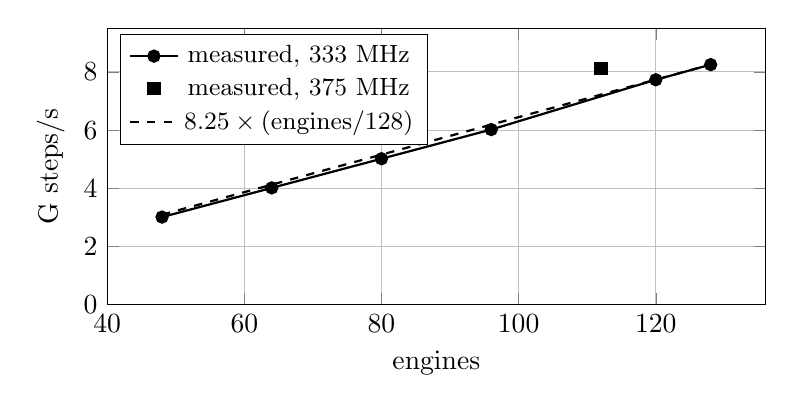
\begin{tikzpicture}
\begin{axis}[
  width=0.82\textwidth,
  height=0.42\textwidth,
  xlabel={engines},
  ylabel={G steps/s},
  xmin=40, xmax=136,
  ymin=0, ymax=9.5,
  grid=major,
  legend style={at={(0.02,0.98)},anchor=north west,font=\small},
]
\addplot[mark=*,thick] coordinates {
  (48,3.0107) (64,4.0137) (80,5.0158) (96,6.018) (120,7.73) (128,8.249)
};
\addlegendentry{measured, $333$~MHz}
\addplot[mark=square*,only marks,thick] coordinates { (112,8.123) };
\addlegendentry{measured, $375$~MHz}
\addplot[dashed,domain=48:128,thick] {0.06445*x};
\addlegendentry{$8.25\times(\mathrm{engines}/128)$}
\end{axis}
\end{tikzpicture}
\caption{ECC2K-130 FPGA engine on AWS F2. The 128-engine image at
  $333$~MHz is $8.25$~G steps/s; the pre-board estimate was
  $5$--$12$~G with a central $8$~G. The measurement landed on the
  central estimate and is a device number, not the estimate reprised.}
\label{fig:fpga}
\end{figure}

Per engine the current revision is $6{,}790$--$6{,}940$ LUTs, $9{,}371$
FFs, 12 RAMB36, 4 URAM and 66 DSPs; the 96-engine image used $62\%$ of
the LUTs and $81\%$ of the block RAM, and block RAM, not logic, is
what bounds the engine count on this part.\art{hdl/ecc2k130/README.md}

\subsection{F2 against the GPU}
\label{sec:fpga-vs-gpu}

At the prices observed on 2026-09-11, an F2 instance at $\$1.980$
on demand or $\$0.709$ spot against an RTX~PRO~6000 at $\$4.14$ and
$\$1.31$ per GPU-hour, the expected $2^{60.9}$ iterations cost about $72{,}400$
F2-hours at the measured $8.25$~G/s, roughly $\$51$k spot, against
$42{,}400$ GPU-hours and $\$56$k spot at the campaign's $14.11$~B/s
collection rate.\footnote{Derived here from the measured rate and the
prices recorded in \texttt{ecc2k130/FPGA-CEILING.md}; the note's own
table priced the hypothetical $8$~B/s image at $\$53$k spot.} The
two platforms are therefore level on cost per solve within the noise
of spot pricing, and the FPGA is about $2$--$5\times$ better per watt
on the note's estimated envelopes ($75$--$150$~W against a $600$~W
board). FPGA workers speak the same client contract as the GPUs and
write the same records, so a collision between an FPGA trail and a
GPU trail is an ordinary merge.

\section{The campaign}
\label{sec:campaign}

$2^{60.9}$ iterations is about five years of single-GPU time at the
campaign's collection rate, so the campaign is collection, not a
solve: a corpus of distinguished points, each
re-walkable from its seed, grown by whatever hardware is cheapest at
the time and merged on arrival. This section records its
configuration, its calibration, its storage protocol and its state.

\subsection{Configuration}

The configuration is one file in the repository; the copy in the
storage bucket is what workers read.\art{ecc2k130/aws/campaign.json}\art{ecc2k130/aws/README.md} Walk: $\sigma$ (Section~\ref{sec:walk-sigma}). \texttt{dpWeight}: 32,
uniform campaign-wide, and a campaign run refuses any other. Batch 16,
256-thread blocks, two resident blocks per SM, $385{,}024$ workers
$=6{,}160{,}384$ logical walks per GPU, $1{,}024$ steps per launch,
checkpoint and upload every 600~s, restart every 48~h. The iteration guard \texttt{maxIters} in the repository file is
$2^{32}$, twelve trail lengths at weight 32; it was $2^{30}$, three
trail lengths, which a model on the measured rates says cut $4.9\%$ of
walks and discarded $15.6\%$ of the fleet's steps until an audit found
it. Whether the bucket copy was raised before the fleet stopped is not
recorded.\art{research/ecc2k130_rho_audit_20260925/README.md} The fields
that define the corpus (workers, batch, geometry, curve, cutoff, walk
and the state-layout knobs) freeze once any slot exists;
\texttt{WITNESS=0} is pinned. The preset is the audited RTX~PRO~6000 build at CUDA~13.3.1 and
\texttt{sm\_120}.\art{ecc2k130/aws/README.md} A checkpoint is about
370~MB (six million walks at 60 bytes).

\subsection{Cutoff 32 and the interval $2^{28.41}$}
\label{sec:campaign-interval}

The planning numbers follow from the cutoff.\art{ecc2k130/aws/README.md, ``The numbers that decide the plan''}
At weight 34 the expected corpus is $2^{35.6}$ records, about $1.7$~TB,
one per $2^{25.27}$ iterations; at weight 32 one report per $2^{28.41}$
iterations, $2^{3.14}=8.8\times$ rarer, so about $2^{32.5}$ records and
$0.19$~TB at the expected work, about 40 points/s, $3.4$~M points/day
and $0.11$~GB/day from a GPU collecting at $14.11$~B/s. The price of a
rarer point is the work left in flight when a collision lands: $43$
GPU-hours per GPU at weight 32 ($6.16$~M walks times $2^{28.41}$
steps), $13\%$ of the expected work at 128 GPUs and more than the
whole expected work at $1{,}024$, against $4.9$ GPU-hours per GPU at
weight 34. The campaign's fleet size never approached the range where
that trade reverses.

The interval itself was measured twice, and the first measurement
was wrong. A fleet-wide ratio of $7.93\cdot10^{15}$ checkpointed
iterations to $31.6$~M uploaded points on 2026-09-15 had been quoted
as $2^{27.9}$ iterations per point. Neither counter was clean: the
checkpoint sum multiplied every slot's per-walk base by the Blackwell
grid constant, inflating the auto-sized Ada slots by the ratio of the
grids (about $26\times$ on an L4-sized grid), and the point total mixed in two retired slots that had walked at weight 34. The
replacement reads from each live worker the client's own two
counters, iterations this run on the grid the client built itself and
points reported over the same interval, frozen at 2026-09-17 18:47~UTC
across 132 workers (Table~\ref{tab:cutoff}).\art{ecc2k130/benchmarks/dp-interval/README.md}
The result, $2^{28.41}=3.56\cdot10^8$, is the same on every hardware
family to $0.04$ in the exponent, and sits $2^{0.60}$ below the naive
binomial $P(\HW\le32)=2^{-29.01}$, as Bailey et al.'s $2^{25.27}$ sits
$2^{0.57}$ below the binomial at weight 34. The correction is
classified as accounting: the walk did not change, the number did,
and the earlier figure is retired rather than averaged.

\begin{table}[t]
\centering
\small
\caption{Iterations per distinguished point at cutoff 32, frozen
  2026-09-17 18:47~UTC. Per-worker spread $0.04$ in the exponent. The
  last column is the median self-reported rate of the family's
  workers on the same day.}
\label{tab:cutoff}
\begin{tabular}{@{}lrrrrr@{}}
\toprule
family & workers & iterations & points & it/point & median B/s \\
\midrule
RTX PRO 6000 (\texttt{g7e}) & 38 & $5.606\cdot10^{15}$ & $15{,}724{,}672$ & $2^{28.41}$ & 14.66 \\
L40S (\texttt{g6e}) & 34 & $2.723\cdot10^{15}$ & $7{,}643{,}600$ & $2^{28.41}$ & 7.47 \\
RTX PRO 4500 (\texttt{g7}) & 48 & $3.081\cdot10^{15}$ & $8{,}640{,}973$ & $2^{28.41}$ & 4.87 \\
CPU & 12 & $2.804\cdot10^{14}$ & $785{,}410$ & $2^{28.41}$ & 2.29 \\
\midrule
all & 132 & $1.169\cdot10^{16}$ & $32{,}794{,}655$ & $\mathbf{2^{28.41}}$ & $\approx1{,}068$ total \\
\bottomrule
\end{tabular}
\end{table}

\subsection{Fleet economics}
\label{sec:campaign-goal28}

Cost is a property of the work, not of the fleet size: at the
2026-09-11 spot price of $\$1.31$ per RTX~PRO~6000 hour the expected
$42{,}400$ GPU-hours are about $\$56$k whether 8 GPUs take 221 days or
512 take $3.4$; on demand the figure is $\$142$k--$\$175$k.\art{ecc2k130/aws/README.md}
What the fleet size buys is the collision-in-flight loss above and the
calendar. The campaign ran mixed families because iterations per
dollar, not iterations per card, is the objective: on 2026-09-18 the best-value quote was an L4 in \texttt{eu-north-1}
at $56\cdot10^{12}$ iterations per dollar against $38\cdot10^{12}$ for the
RTX~PRO~6000 and $28\cdot10^{12}$ for the RTX~PRO~4500, and at that
quote a full reference walk costs about
$\$38$k.\art{ecc2k130/aws/RESEARCH-CREDITS.md} The per-SKU rates
behind those ratios are measured, not list: L40S $8.84$~B/s with
\texttt{clmad}, L4 $2.49$, T4 $0.53$ without it.\art{ecc2k130/ADA-L4-L40S.md}\art{ecc2k130/T4-G4DN.md}

The RTX~PRO~4500 is the instructive case. Its measured $5.107$~B/s on
the shipping walk is exactly what the 6000's rate predicts from SM
count and clock ($14.64\times82/188\times1.95/2.44=5.10$), and at that rate the 6000 wins per dollar by $1.2$--$1.3\times$; the
break-even against the 6000's shipping rate is $6.2$--$6.6$~B/s in the
two cheapest regions and $8.8$ in the third, figures the note says
must be redone with both cards on their best
builds.\art{ecc2k130/RTX-PRO4500.md} That
is why a $12$~B/s goal was set for the card and why the $x$-only
bridge map of Section~\ref{sec:walk-bridge} was pursued there rather
than on the 6000: a power-capped die rewards fewer instructions per
step more than a pipe-bound one does. The separate goal of $28$~B/s on
one 6000 was priced below the pipe (Section~\ref{sec:floor}) and its
grid and occupancy screens, run on an RTX~PRO~4500 because no 6000
could be allocated, found nothing faster than the shipping
configuration.\art{ecc2k130/GOAL28-RESULTS.md}

A power survey closes the loop: on the 6000 the $20$~B/s build drew
$583$~W for $34.4$~M updates per joule and a fused-pass variant
$544$~W for $37.0$~M/J in the same session, $1.072\times$ per joule in
five paired repetitions against a $1.03$ target; per joule, not per
second, is the figure that transfers to a $165$~W card, and the model,
calibrated on the 4500's $5.107$ and $5.552$~B/s receipts (ratio error
$+2.6\%$), predicts $7.2$--$7.4$~B/s for the fused build
there.\art{ecc2k130/POWER-BOUND.md} That prediction is owed a
measurement; the bridge map arrived first.

\subsection{Storage, seeds and certification}
\label{sec:campaign-storage}

A record is 32 bytes: a little-endian 64-bit seed and the canonical
normal-basis $x$ of the endpoint, three 64-bit words; no scalar
coefficients are stored, they are rebuilt by replay. The seed is \texttt{run id (16) $\|$ walk index (32) $\|$ restart
counter (16)} with run id $=$ slot $+1$; a splitmix64 finaliser
expands it to the 128-bit $c$ of the start point. Two contributors who
pick different run ids never start the same walk (independently
seeded walks can still meet, which is the point), and a permanent seed
registry does compare-and-set across providers (Modal GPU runs are ids
8000--8999, CPU sidecars 9000--9999); a race test with eight claimants
acquired exactly one.\art{ecc2k130/CERTIFICATION.md}\art{ecc2k130/SEED-IDENTITY.md}\art{research/ecc2k130_rho_audit_20260925/README.md, ``Seeds''}\art{ecc2k130/aws/README.md}

Uploads are ordered so that no pointer ever names data that is not
there: payloads before their commit manifests, both before checkpoint
publication. Strict manifests bind curve, cutoff, guard, seed and key
semantics, worker geometry, source hash, worker binary hash and
replay binary hash, and every immutable payload carries its SHA-256.
Slot ownership is one S3 object per slot claimed with a conditional
put on the ETag, a 60~s heartbeat and a 180~s lease; checkpoints are
content-addressed and the owner-checked heartbeat publishes the
pointer, so a stale worker can leave orphaned blobs but cannot commit.
The note is explicit that this is integrity against failure, not
authentication against an actor able to rewrite both data and
manifests.\art{ecc2k130/CERTIFICATION.md}\art{ecc2k130/aws/README.md, ``Slots''}

Merging buckets records by a hash of the key limbs (the first layout
used the key's low bits) into $4{,}096$ files, sorts, drops exact duplicates (the client store, the database primary
key and the merge are three layers; $9.95$~M re-reports had been
dropped by 2026-09-25) and reports equal keys with different seeds.
Such a pair goes into a two-record file and to the CPU client, which
re-walks both trails, aligns Frobenius and negation, and verifies
$[k]P=Q$; a $\mathrm{GF}(2^{41})$ pair with known seeds that recovers
$k=369250562913$ is the local acceptance fixture. An exhaustive check of $76{,}904{,}684$ step multisets confirms that
no multiset of at most 32 $\sigma$-walk steps closes an orbit, so no
short fruitless cycle exists; a trail crossing itself at random is
estimated at about $2^{-65}$ per trail, about $10^{-10}$ over the
campaign, and the iteration guard releases such a
walk.\art{ecc2k130/CERTIFICATION.md}\art{research/ecc2k130_rho_audit_20260925/README.md}\art{ecc2k130/aws/README.md}

The public dashboard publishes aggregates only: not point keys,
coefficients, seeds or database locations.\art{docs/ecc2k130-status/README.md}\art{scripts/rho_status/README.md}

\subsection{State}
\label{sec:campaign-state}

The campaign was created on 2026-09-11. Its fleet on 2026-09-17 was about 133 workers (the 132 with enough
points to calibrate are in Table~\ref{tab:cutoff}), producing about
$2{,}600$ points/s by the ingest's count; the ingest path was re-engineered that week from one object
at a time ($2{,}450$ records/s, below production) to a threaded loader
measured at $137{,}753$ rows/s, and a five-and-a-half-hour blind spot during a key layout change was
recovered in 23 minutes ($4{,}321$ objects,
$63{,}351{,}803$ rows, zero failed), taking the store from $67.6$~M to
$124.3$~M points.\art{ecc2k130/aws/README.md} On 2026-09-18 the spot market reclaimed every worker and the cloud
account was placed on an account-verification (risk) hold that has
blocked new instance launches since; collection continued at a small
scale on another provider. Its first four GPU runs reused the run ids
of the first four slots by mistake and re-walked them ($813$k of one
run's $912$k records byte-identical to the slot they replayed, all
dropped as re-reports, and an inadvertent end-to-end replay check);
later runs use the reserved ids
8000--8999.\art{ecc2k130/aws/ACCOUNT-HOLD.md}\art{ecc2k130/README.md, ``Collecting for the campaign from Modal''}

Table~\ref{tab:state} gives two snapshots: the audited one of
2026-09-25, while a small fleet was still walking, and the published
feed of 2026-10-10, by which time the last point had landed
(2026-10-07) and no slot was walking; the sustained peak and the
mean trail length in the caption are from the
audit.\art{research/ecc2k130_rho_audit_20260925/live_status_20260925T050509Z.json}\art{paper/ecc2k130/data/status_20261010T154157Z.json}\art{research/ecc2k130_rho_audit_20260925/README.md}
No collision is the expected state: $2^{56.68}$ iterations is $5.4\%$
of $2^{60.9}$, and the probability of no collision after a fraction
$c$ of the expected work is about $\exp(-\pi c^2/4)$, here $0.998$.
Collection is paused, not finished: every slot's checkpoint and the
corpus are intact, and a worker that resumes a slot continues its
walks from the checkpoint.

\begin{table}[t]
\centering
\small
\caption{Campaign state at the audited snapshot of 2026-09-25
  05:05~UTC and at the published feed of 2026-10-10 15:42~UTC. The pooled iterations-per-point ratio is below $2^{28.41}$, partly
  because the corpus still holds weight-34 records from the first two
  slots; the mean length of walks that ended by 2026-09-25 is
  $2^{28.34}$. Sustained production peaked at about $842{,}000$ points
  per hour on 2026-09-23, about $83$~B it/s.}
\label{tab:state}
\begin{tabular}{@{}lrr@{}}
\toprule
 & 2026-09-25 & 2026-10-10 \\
\midrule
distinguished points stored & $367{,}123{,}410$ & $485{,}528{,}850$ \\
iterations (checkpointed) & $2^{56.38}$ & $2^{56.68}$ \\
share of expected work & $4.4\%$ & $5.4\%$ \\
collisions & 0 & 0 \\
duplicate re-reports dropped & $9{,}953{,}494$ & $14{,}153{,}833$ \\
slots / walking / off-weight & 195 / 2 / 7 & 227 / 0 / 7 \\
points in the last 24~h & $741{,}048$ & 0 \\
walk rate over the last hour & $3.65$~B it/s & 0 \\
last point stored & --- & 2026-10-07 14:41 \\
\bottomrule
\end{tabular}
\end{table}

\section{Structural alternatives, measured}
\label{sec:alternatives}

Every row above is engineering against a fixed exponent. Three
threads asked whether the exponent could move for this curve, in the
same accounting, and each is reported here with its measurement
because a later reader who rediscovers the idea should find the
number rather than the folklore. None changed the campaign.

\subsection{Index calculus on the Koblitz curve}
\label{sec:alt-ic}

Index calculus on $E(\FF_{2^n})$ decomposes a random point into $m$
factor-base points through Semaev's summation
polynomials~\cite{semaev2004,gaudry2009,diem2011,faugere2012,petitquisquater2012,galbraithgebregiyorgis2014};
on a Koblitz curve the factor base can be taken Frobenius-stable so
that columns are orbits, saving a factor $n$ in relations and $n^2$ in
linear algebra against rho's $\sqrt{2n}$. Two structural facts about
$n=131$ come first. In a normal basis the Frobenius is a coordinate
permutation, so a Frobenius-stable subspace is an
$\FF_2[t]/(t^n-1)$-submodule, a binary cyclic code of length $n$, and
at $n=131$ (and $n=163$) $2$ is primitive modulo $n$, so $t^n-1$ has
exactly two factors and the only stable subspaces have dimension
$0,1,130,131$. The usual subspace construction is empty at exactly the interesting
sizes; forced onto the 130-dimensional subspace, the orbit trick is a
net loss of $57$--$96$ bits for
$m\in\{2,\ldots,5\}$.\art{RESEARCH_KOBLITZ_INDEX_CALCULUS.md}\art{autoresearcher:ledger/evidence/EV-FROB-d336b0.yaml}
The Couveignes--Lercier elliptic-period alternative needs an auxiliary
curve over $\FF_2$ with $n\mid\#E'(\FF_2)$, and Hasse gives at most
5.\art{RESEARCH_KOBLITZ_INDEX_CALCULUS.md} What survives is a
weight-bounded base $\{R:\HW(x_R)\le w\}$ in the normal basis, which
is Frobenius-stable for every $n$, is the predicate the walk already
computes, and is not a low-degree algebraic condition, so only a
solver that does not need linearity can use it.

\paragraph{SAT decomposition.} Chaining Semaev's $S_3$ through the
intermediate sums, with squaring free, encodes a $k$-point
decomposition as a CNF whose multiplications cost the generated
Karatsuba circuit's gates ($15{,}588$ at $n=131$ against $2.2$ million for the definition). With $k=3$, $w=3$ and CryptoMiniSat the median solve is $0.11$~s at
$n=9$ and $2.64$~s at $n=11$; at $n=23$ no instance finished, one
running 25 minutes without returning: roughly $2^{2.3}$ per field bit
over that range, from three points.\art{ecc2k130/README.md, ``Index calculus: SAT point decomposition''}

\paragraph{The compact-orbit ladder.} A separate line of work solves rungs of the same curve family ($a=0$,
the ECC2K-130 equation) with a four-summand decomposition, at $n=41$
and $53$ over 85- and 220-column bases and at $n=61,71,73$ over a
600-column base, fully charged, and fits the rank cost. Table~\ref{tab:ic-rungs}
is the measured cost and its extrapolation to $n=131$ under the fit
$\text{probes/relation}\approx C\,r/(n^2K^2)$ with
$C=1$.\art{RESEARCH_ECC2K130_IC_FEASIBILITY.md} The fitted $C$ ($0.33$ at $n=61$, $1.51$ at $n=71$, $1.27$ at $n=73$,
recomputed here from the exact subgroup orders) disagrees with the
structural model's $0.25$ by a factor of $1.3$ to $6$, and the note
records the gap as open; the extrapolation uses $C=1$, between the
structural $0.25$ and the fitted $1.3$--$1.5$ of the two largest
rungs.

\begin{table}[t]
\centering
\small
\caption{Four-summand compact-orbit index calculus on the ECC2K-130
  curve family, single thread, $K=600$ columns, precompute fully
  charged (left), and the extrapolation to $n=131$ ($r=6.8\cdot10^{38}$)
  at $1.85\cdot10^6$ probes/s (right). The minimum base for one
  expected four-tuple per point is $B>r^{1/4}=5.1\cdot10^9$ points,
  $K\ge2\cdot10^7$.}
\label{tab:ic-rungs}
\begin{tabular}{@{}rrrr@{}}
\toprule
$n$ & $r$ (bits) & rank wall & probes/relation \\
\midrule
61 & 47.2 & $13.1$~s & $\sim4\cdot10^4$ \\
71 & 52.3 & $1{,}485$~s & $\sim4.6\cdot10^6$ \\
73 & 56.3 & $18{,}398$~s & $5.7\cdot10^7$ \\
\bottomrule
\end{tabular}
\hspace{1.5em}
\begin{tabular}{@{}rrrr@{}}
\toprule
$K$ & probes/relation & total probes & core-years \\
\midrule
$600$ & $1.1\cdot10^{29}$ & $6.6\cdot10^{31}$ & $1.1\cdot10^{18}$ \\
$10^6$ & $4.0\cdot10^{22}$ & $4.0\cdot10^{28}$ & $6.8\cdot10^{14}$ \\
$10^9$ & $4.0\cdot10^{16}$ & $4.0\cdot10^{25}$ & $6.8\cdot10^{11}$ \\
$10^{12}$ & $4.0\cdot10^{10}$ & $4.0\cdot10^{22}$ & $6.8\cdot10^{8}$ \\
\bottomrule
\end{tabular}
\end{table}

The verdict is in the unit of the rest of the paper. Rho at $2^{60.9}$ iterations on one RTX~PRO~6000 is about five
GPU-years at the campaign's $14.11$~B/s. Four-summand index calculus
has total work about $r/(n^2K)$ probes: at $K=10^9$ that is
$4\cdot10^{25}$, some $2\cdot10^7$ times rho's iteration count with one
probe counted as one step (uncalibrated), and the base at which the precompute alone equals
rho is $K\approx1.8\cdot10^{16}$ columns, beyond any linear algebra
contemplated. The rungs that beat rho do so only in the online class
after a precompute that is excluded from the clock (at $n=73$, $18{,}400$~s of precompute against $46$~s of rho online, a
$400\times$ total-work deficit traded for a $185\times$ exploratory
online wall ratio on one frozen target, on a shared host), and with
the precompute charged the method spends $26$--$1{,}200\times$ more
probes than one rho solve takes steps on every rung, again
uncalibrated.
Beating rho on total work needs a relation-shape change (five- or
six-summand relations, whose per-point yield scales as $B^5/(120r)$),
not engineering, and that oracle is unmeasured.\art{RESEARCH_ECC2K130_IC_FEASIBILITY.md, §3--4}
In this repository's boundary ledger the Koblitz rows at a 39-bit
subgroup run from $S=\text{ops}/\sqrt r=58.8$ ($300\times$
signed-Frobenius rho) for the plain three-summand meet-in-the-middle
oracle down to $5.12$ ($26\times$; $5.92$ and $30\times$ on
re-measurement) for a balanced two-summand base; the secondary
complete-CPU panel on disjoint public points at $n=37,41,53$ has rho
ahead in every cell.\art{research/notes/index-calculus/RESEARCH_IC_BOUNDARY_LEDGER.md}\art{docs/ic/BOUNDARY_TARGETS.md}

\subsection{Point decomposition against the per-call budget}
\label{sec:alt-pdp}

The sibling library prices the same question from the other end:
given rho's $2^{60.81}$ orbit-walk iterations, how fast must one
$m$-summand decomposition be for index calculus to fit inside that
budget, and how fast is the best one measured? With a base of
$2^\ell$ points, $m=4$ at $\ell=29$ needs $2^{48.6}$ decompositions and
$2^{60.0}$ of linear algebra, leaving $2^{12}$ rho-iterations per
decomposition; $m=5$ at $\ell=28$ leaves $2^{33}$; $m=6$ at $\ell=24$
leaves $2^{37}$; $m=3$ has no budget at all because the linear algebra
alone exceeds rho. The best measured decomposition is the
non-algebraic meet-in-the-middle at exponent $\lceil m/2\rceil$ in
$\ell$, and extrapolated to $n=131$ it is $2^{58}$, $2^{84}$ and $2^{72}$
for $m=4,5,6$: $35$--$51$ bits over the budget. Algebraic solvers land far higher: SAT fits at $2^{4}$ ($m=3$) to
$2^{7}$ ($m=4$) per unit of $\ell$, msolve grows faster still, and
WDSat at about $2^{3}$, the exhaustive-search exponent. An attack needs a decomposition about $2^{35}$--$2^{50}$
times faster than meet-in-the-middle at $\ell\approx25$--$30$, which is
the obstruction that stops Wagner's $k$-tree from applying to elliptic
curves; the trace-homomorphism clause that halves UNSAT conflicts is a
constant, not an exponent.\art{cryptanalysis:experiments/pdp-scaling/README.md}
A Riemann--Roch (Nagao) oracle on the real curve was measured at
factor-base dimensions 4--8 and its derived product law
($\text{relations}\times\text{targets}\times\text{oracle}=m\cdot2^{131}$)
leaves even a free oracle above rho at $m=3$ ($2^{68.6}$) and below it
only from $m=4$ ($2^{56.4}$, leaving $2^{4.4}$ of headroom for the
oracle itself), where no measured oracle comes close.\art{autoresearcher:ledger/evidence/EV-ICPERF-10c5fc.yaml}

\subsection{What the negatives say}

Each alternative was carried to a measurement and each landed above
rho by a margin that is a change of exponent, not of constant. The
honest summary for ECC2K-130 is that the generic-group floor,
$\sqrt{\pi\ell/(2\cdot262)}$ class-walk steps, is still the number
the campaign is walking toward, and that the only lever that has
moved in this work is the cost of one step.

\section{Related work}
\label{sec:related}

\paragraph{The 2009 attempt.} Bailey et al.~\cite{bailey2009} fixed
the iteration function this campaign walks, $R\mapsto\sigma^j(R)+R$
with $j$ from the weight of $x$, the weight-34 distinguished-point
rule, and the $2^{60.9}$ budget, and reported per-platform rates on
Core~2 (533 cycles per iteration with 128-bit vectors), Cell, GPUs,
FPGAs~\cite{fan2010fpga} and ASIC estimates; their SHARCS
paper~\cite{bailey2009sharcs} priced the whole Certicom ECC2 list.
Bos, Kleinjung, Niederhagen and Schwabe's Cell
implementation~\cite{bos2010cell} is the bitsliced lineage this
client's CPU and first GPU backends belong to. The type-II
optimal-polynomial-basis multiplication of Bernstein and
Lange~\cite{bernsteinlange2010onb} is used verbatim; the conversion
networks generated here match their hand-designed chains to within a
few instructions (Section~\ref{sec:arith-bitsliced}). Bernstein's bit
operation counts for binary multiplication~\cite{bernstein2009batch}
are the reference the three-input-logic finding is measured against.
Bernstein et al.'s later FPGA designs~\cite{bernstein2016fpga}, which
set the current size record for a completed binary-curve computation
by solving a $2^{117.35}$-order instance on sect113r2 and were
extrapolated to a 127-bit field, are the calibration for the pre-board
estimate of Section~\ref{sec:fpga}, which the measurement then met.
Harley's group solved ECC2K-95 in 1998 and ECC2K-108 in April 2000,
the latter with about $1{,}300$ volunteers' machines over four
months~\cite{harley1998,harley2000}; those two are the only Koblitz
challenges completed, and their walks are the ancestors of the one in
Section~\ref{sec:walk-sigma}.

\paragraph{Rho on automorphism classes.} The $\sqrt{2m}$ saving from
Frobenius and negation on Koblitz curves is due to Wiener and
Zuccherato~\cite{wienerzuccherato1998} and Gallant, Lambert and
Vanstone~\cite{glv2000}, generalised by Duursma, Gaudry and
Morain~\cite{duursma1999}. Teske's $r$-adding walks~\cite{teske2001}
and the Bernstein--Lange--Schwabe treatment of fruitless cycles under
the negation map~\cite{bls2011} are the background to
Section~\ref{sec:walk-table}; the cycle classes measured there are the
$\tau$-relation analogue, and the measured walk constants of
Table~\ref{tab:walkconst} are, to our knowledge, the first reported
for this branch distribution on this family. The distinguished-point
method is van Oorschot and Wiener's~\cite{vanoorschot1999}. The 112-bit
prime-field record of Bos et al.~\cite{bos2012ps3} is the nearest
completed computation in scale.

\paragraph{Index calculus on binary curves.} Semaev's summation
polynomials~\cite{semaev2004}, Gaudry's and Diem's index
calculus~\cite{gaudry2009,diem2011}, the Faug\`ere--Perret--Petit--Renault
and Petit--Quisquater analyses of Weil-descent
systems~\cite{faugere2012,petitquisquater2012} and Galbraith and
Gebregiyorgis's characteristic-two
algorithms~\cite{galbraithgebregiyorgis2014} are the methods
Section~\ref{sec:alternatives} prices on this curve. The structural
closure at $n=131$ (no Frobenius-stable subspace of intermediate
dimension) is elementary once the normal basis is in view, and the
measured ladder confirms that the surviving weight-bounded bases do
not reach the budget.

\paragraph{Measurement discipline.} The companion
paper~\cite{ecdlppaper} states the boundary-unit-table-class rule and
applies it across rho, baby-step giant-step, kangaroo and prime-field
index calculus; this paper is its ECC2K-130 chapter at full length.

\section{Conclusion}
\label{sec:conclusion}

Four statements survive the accounting.

First, ECC2K-130 is an arithmetic problem at a known exponent, and the
exponent did not move. Index calculus on the curve, priced end to
end, is $10^7$ times rho at the challenge size with four-summand
relations; the best measured decomposition is $35$--$51$ bits short of
the per-call budget; the Frobenius-stable subspaces that the
literature's construction needs do not exist at $n=131$. The number
the campaign walks toward is still $\sqrt{\pi\ell/(2\cdot262)}$ class
steps.

Second, the cost of a step on a GPU was measured against a floor
written first. Sixteen paired rungs took one RTX~PRO~6000 from
$0.85$ to $14.64$ billion complete iterations per second with the
campaign's $\sigma$-walk, later $\sigma$-walk builds reached $15.88$,
a table walk reached $20.08$ as a rate, and the roofline of that build
puts the logic pipe at $91\%$ and the carry-less unit at $73\%$ of
saturation. Twenty-eight on one card is
below both pipes for any walk that performs one affine addition per
step; thirty is a two-card number. A $17.0$~B/s target declared before
a build declined a $16.56$~B/s result, which is what a declared target
is for.

Third, the step count is measured, not assumed. The campaign's
$\sigma$-walk costs $2^{60.91}$--$2^{60.92}$ iterations, the 2009
estimate within its own precision; the table walk's cheaper constant
was paid back several times over by fruitless cycles until the rule
was fixed, and its projected $0.81$--$0.86$ cost per solve awaits the
paired run that would confirm it. An FPGA engine designed from the
same model measured $8.25$~G steps/s on one F2 against a pre-board
central estimate of $8$, level with the GPU on cost per solve.

Fourth, the campaign is a corpus, and the corpus is honest. One
report per $2^{28.41}$ iterations at cutoff 32, a figure that replaced
a wrong $2^{27.9}$ and says so; $486$ million points and $2^{56.68}$
iterations with no collision, $5.4\%$ of the expected work, every
record re-walkable from its seed and every rate in this paper
re-walked before it was recorded. The fleet that produced most of it
was reclaimed on 2026-09-18, the last point landed on 2026-10-07, and
collection is paused. Whether the remaining $94.6\%$ is walked is a
question of money, not of mathematics; this paper's contribution is
to have priced it.

\appendix
\section{Reproduction}
\label{app:repro}

All commands run from the repository root unless a directory is
named. CUDA rows need the card named in the row; the host checks do
not.

\paragraph{Field, walk and solver.}
{\small\begin{verbatim}
cd ecc2k130 && make generate && make test        # 52 checks, GF(2^23..131)
make break-small   # planted logs, GF(2^41)
python3 ecc2k130/examples/rho_toy.py   # the walk on GF(2^23)
\end{verbatim}}

\paragraph{GPU rates (RTX PRO 6000 unless noted).}
{\small\begin{verbatim}
make -C ecc2k130 bench-rtx-pro6000   # audited sigma preset, 14.64 B/s
make -C ecc2k130 audit-rtx-pro6000   # same, with DP34 collection
make -C ecc2k130 gpu-rtx-pro6000-20b   # one-block table walk, 20.08 B/s
make -C ecc2k130 gpu-rtx-pro6000-sigma-fused      # 15.44 B/s
make -C ecc2k130 gpu-b200-19b   # B200 autosweep arm, 19.40 B/s
make -C ecc2k130 bench-local-packed   # RTX PRO 4500 bridge map, 12.50 B/s
python3 ecc2k130/benchmark_instance.py   # concurrent-instance accounting
\end{verbatim}}
Every rate is a paired comparison; the candidate/control pairs,
raw samples and re-walk logs are in the \texttt{ecc2k130/benchmarks/}
directory each note links.

\paragraph{Walk constant and cycles.}
{\small\begin{verbatim}
make -C ecc2k130 test-cycle-rule   # 19,200 tau-cycles refused
# scatter runs and c measurements: ecc2k130/WALK-CONSTANT.md, section 4 and 11.6
\end{verbatim}}

\paragraph{FPGA.}
{\small\begin{verbatim}
cd hdl/ecc2k130 && python3 ecc2k_ref.py check && make   # vectors, testbenches
make rate   # 6,144 steps, clk/step
cd aws && NENG=128 CLK_MHZ=333 ./build_afi.sh push && ./build_afi.sh launch
\end{verbatim}}

\paragraph{Campaign.}
{\small\begin{verbatim}
cat ecc2k130/aws/campaign.json   # frozen configuration
ecc2k130/benchmarks/dp-interval/   # 2^28.41 calibration, raw TSV
ecc2k130/CERTIFICATION.md   # storage and replay protocol
research/ecc2k130_rho_audit_20260925/   # live snapshot and audit
\end{verbatim}}

\paragraph{Alternatives.}
{\small\begin{verbatim}
cd ecc2k130/codegen && \
  python3 indexcalc.py --m 11 --points 3 --weight 3 --trials 5
RESEARCH_ECC2K130_IC_FEASIBILITY.md   # compact-orbit ladder, n=131
cryptanalysis:experiments/pdp-scaling/   # decomposition budget
\end{verbatim}}


\bibliographystyle{plainnat}
\bibliography{ecc2k130}

\end{document}
